% The appendix or appendices should contain your group meeting minutes and any additional raw material that is referred to in the text (e.g. data from requirements gathering, paper prototypes etc.)

\section{Prototyping}
\subsection{AR Prototypes}
\subsubsection{Vulforia}
\begin{figure}[H]
\centering  
\begin{tabular}{cc}
  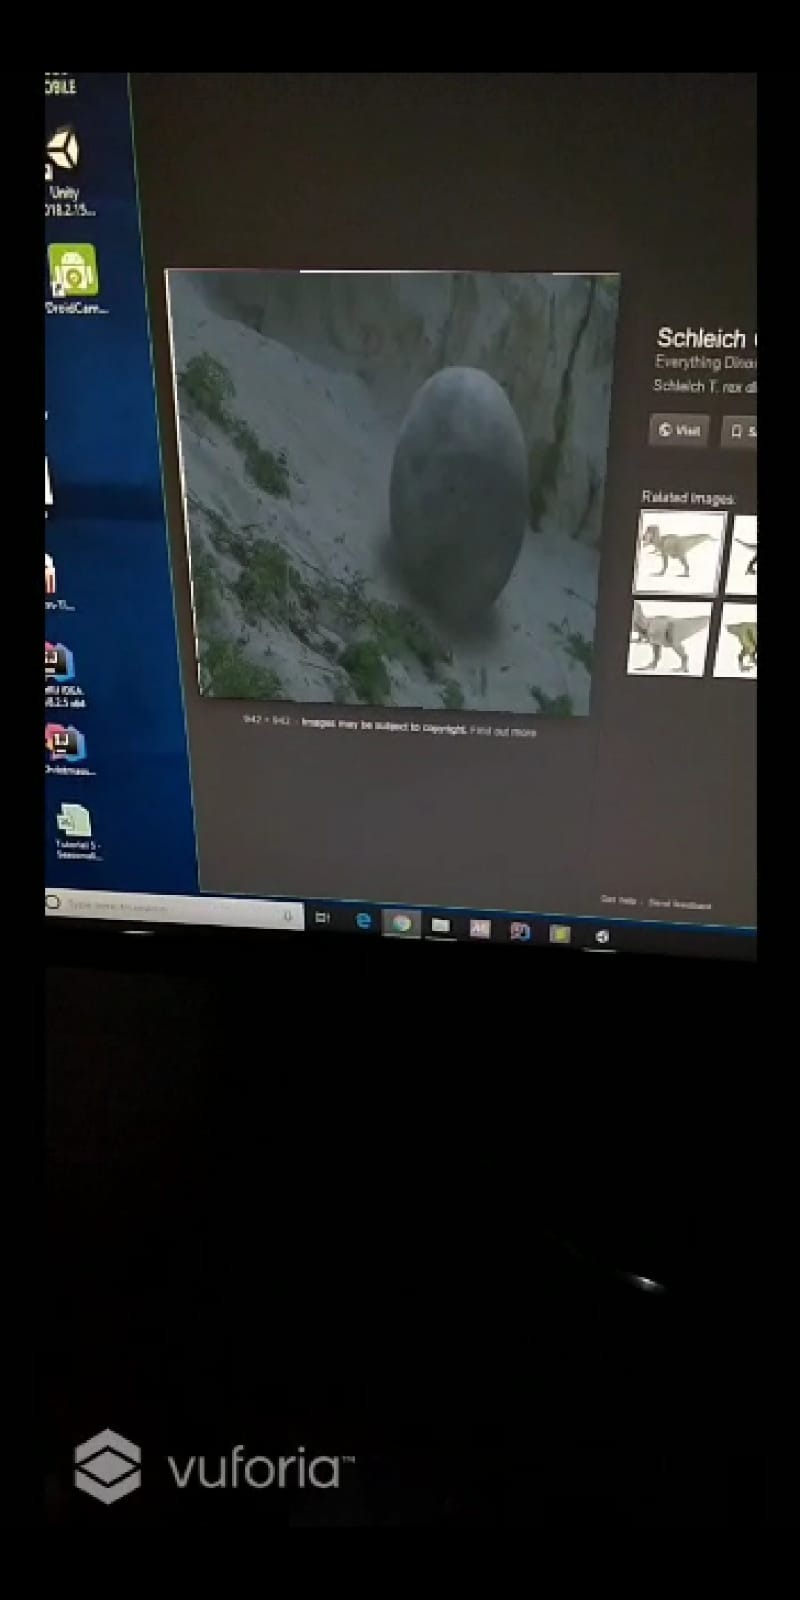
\includegraphics[width=60mm, height=100mm]{prototypes/ar/vulforia/1.jpeg} &   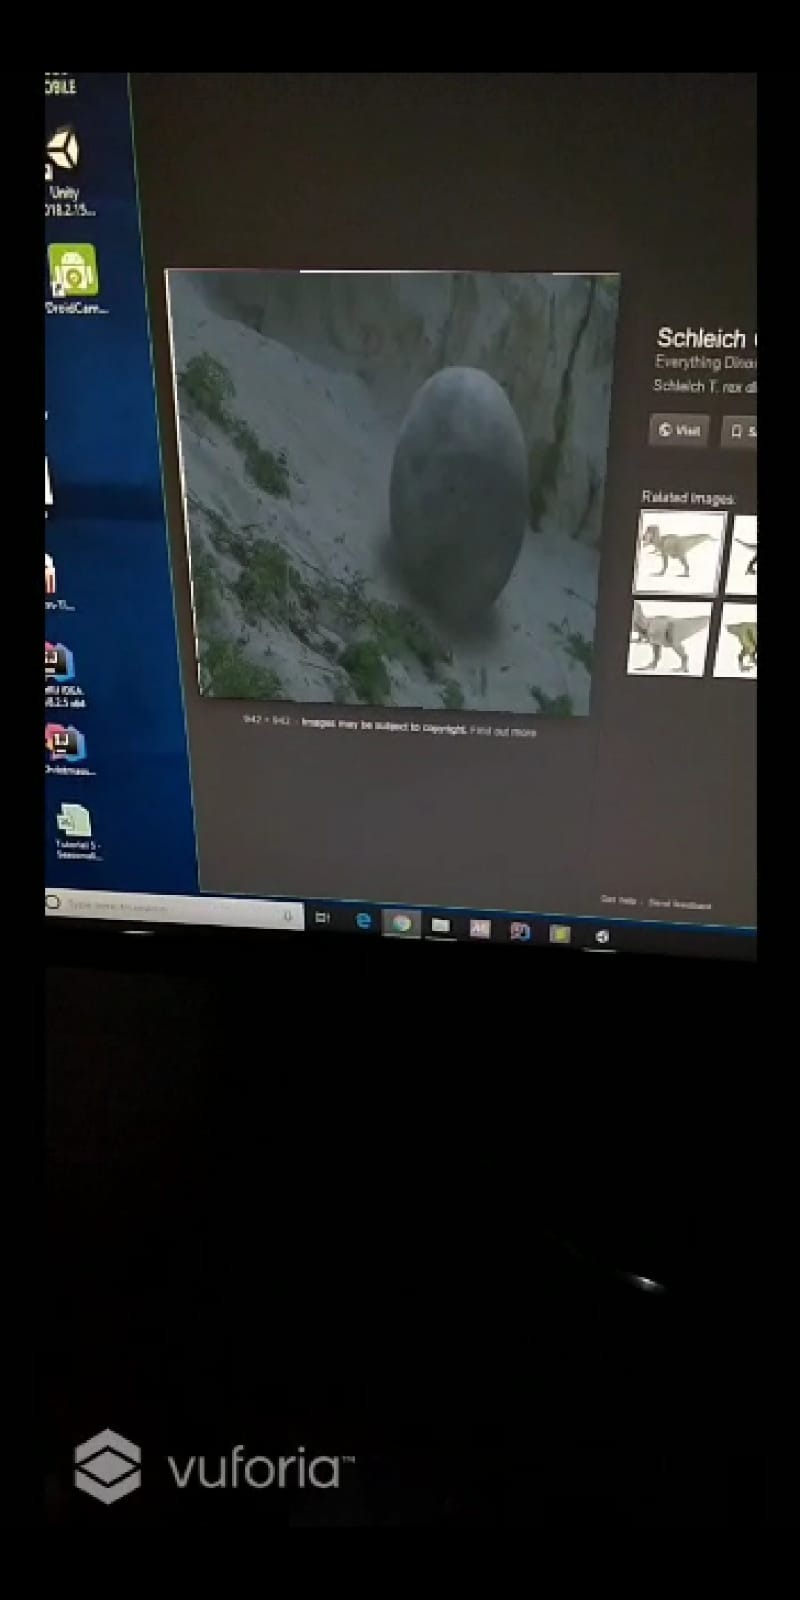
\includegraphics[width=60mm, height=100mm]{prototypes/ar/vulforia/2.jpeg} \\
(a) Camera over image & (b) Video superimposed on top of image\\[6pt]
\end{tabular}
\caption{Vulforia prototyping on Android device}
\label{fig:vulforia}
\end{figure}

\newpage
\subsubsection{ARKit}
\begin{figure}[H]
\centering  
\begin{tabular}{cc}
  \includegraphics[width=60mm, height=100mm]{prototypes/ar/ios/1.png} &   \includegraphics[width=60mm, height=100mm]{prototypes/ar/ios/2.png} \\
(a) Camera over image & (b) Image recognised and displaying information \\[6pt]
\multicolumn{2}{c}{\includegraphics[width=60mm, height=100mm]{prototypes/ar/ios/3.png} }\\
\multicolumn{2}{c}{(c) Image scanned before; showing the green tick}
\end{tabular}
\caption{ARKit prototyping on iOS device}
\label{fig:ARKit}
\end{figure}

\newpage
\subsubsection{ARCore}
\begin{figure}[H]
\centering  
\begin{tabular}{cc}
  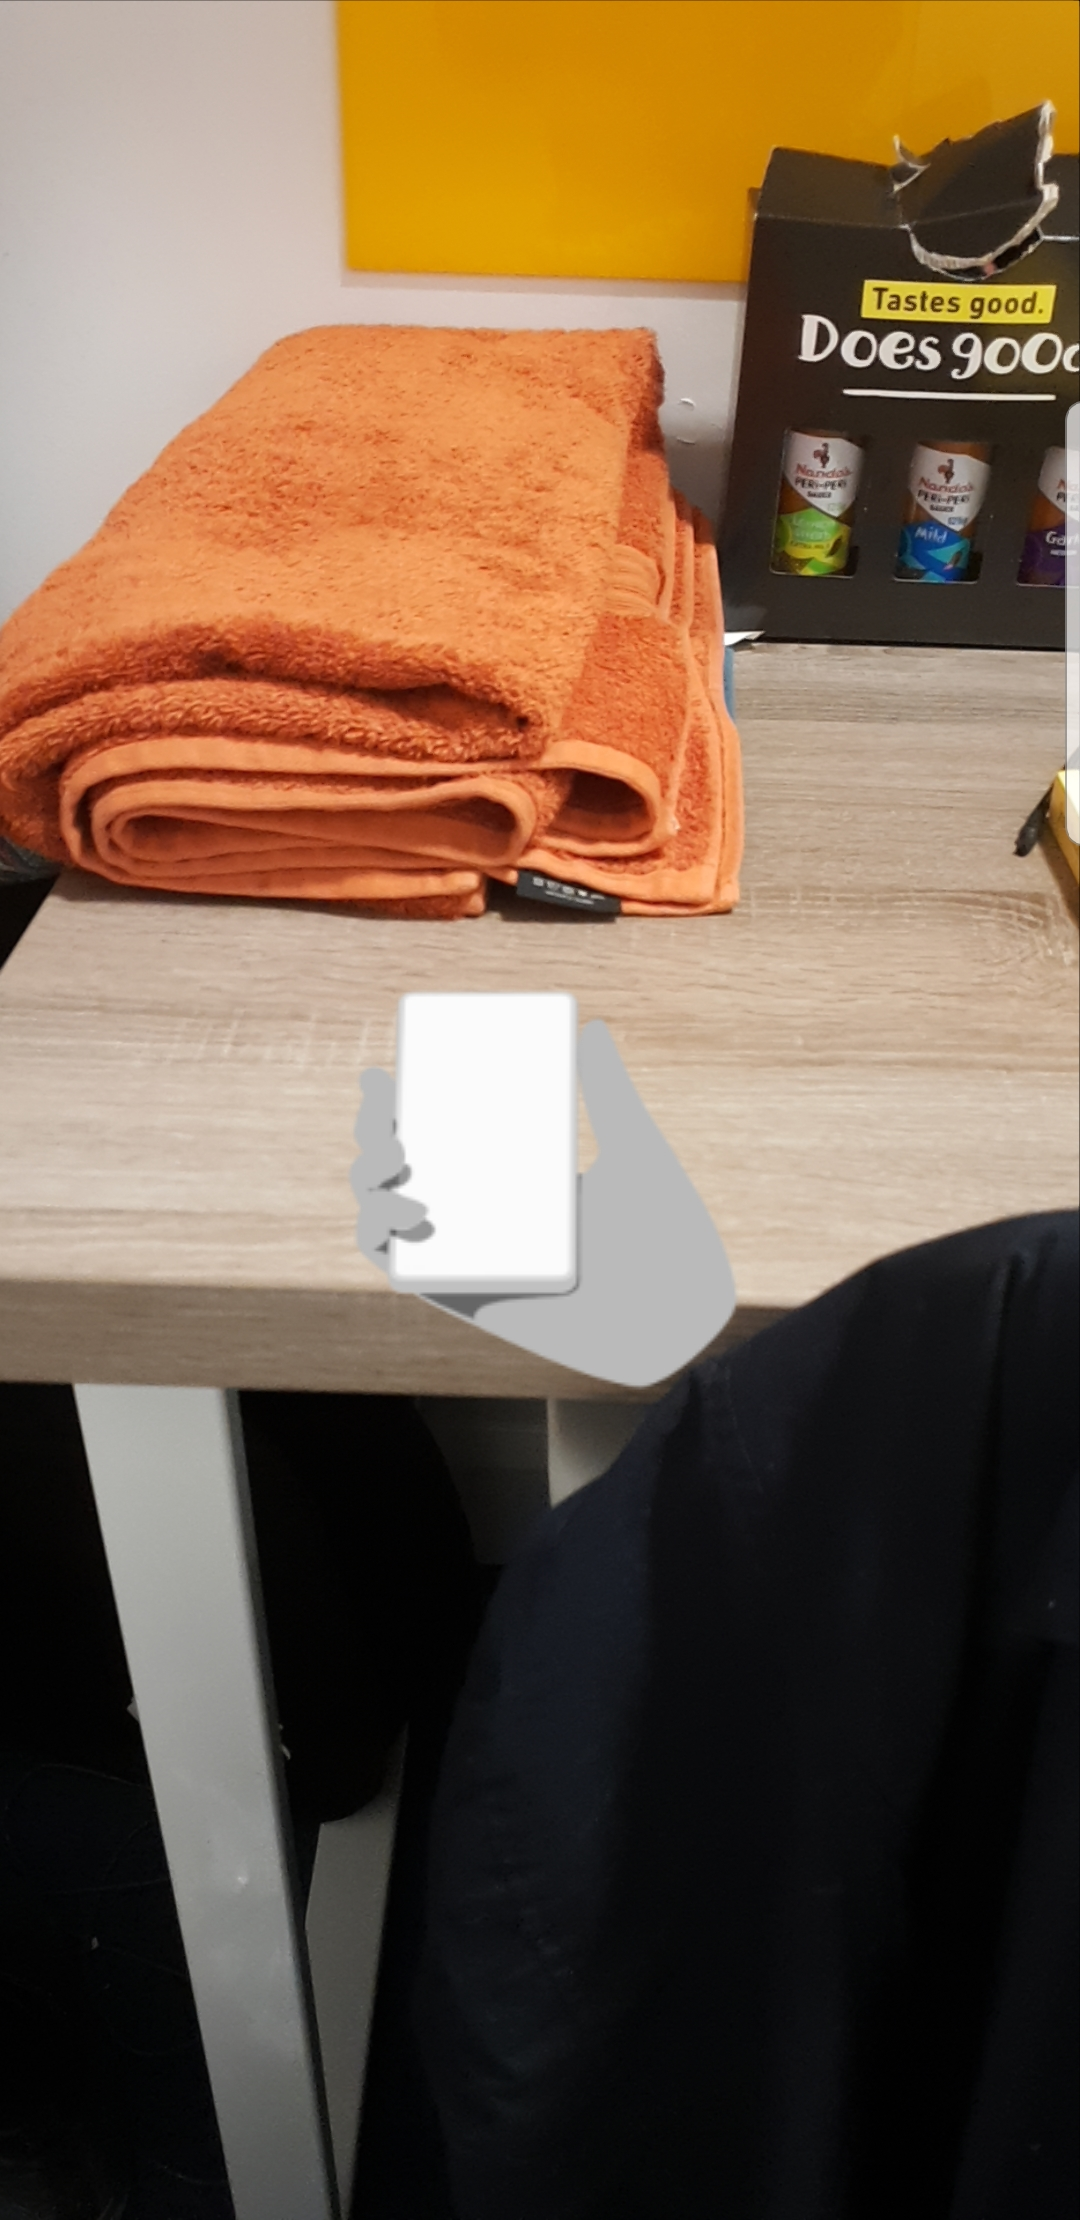
\includegraphics[width=60mm, height=100mm]{prototypes/ar/android/1.jpg} &   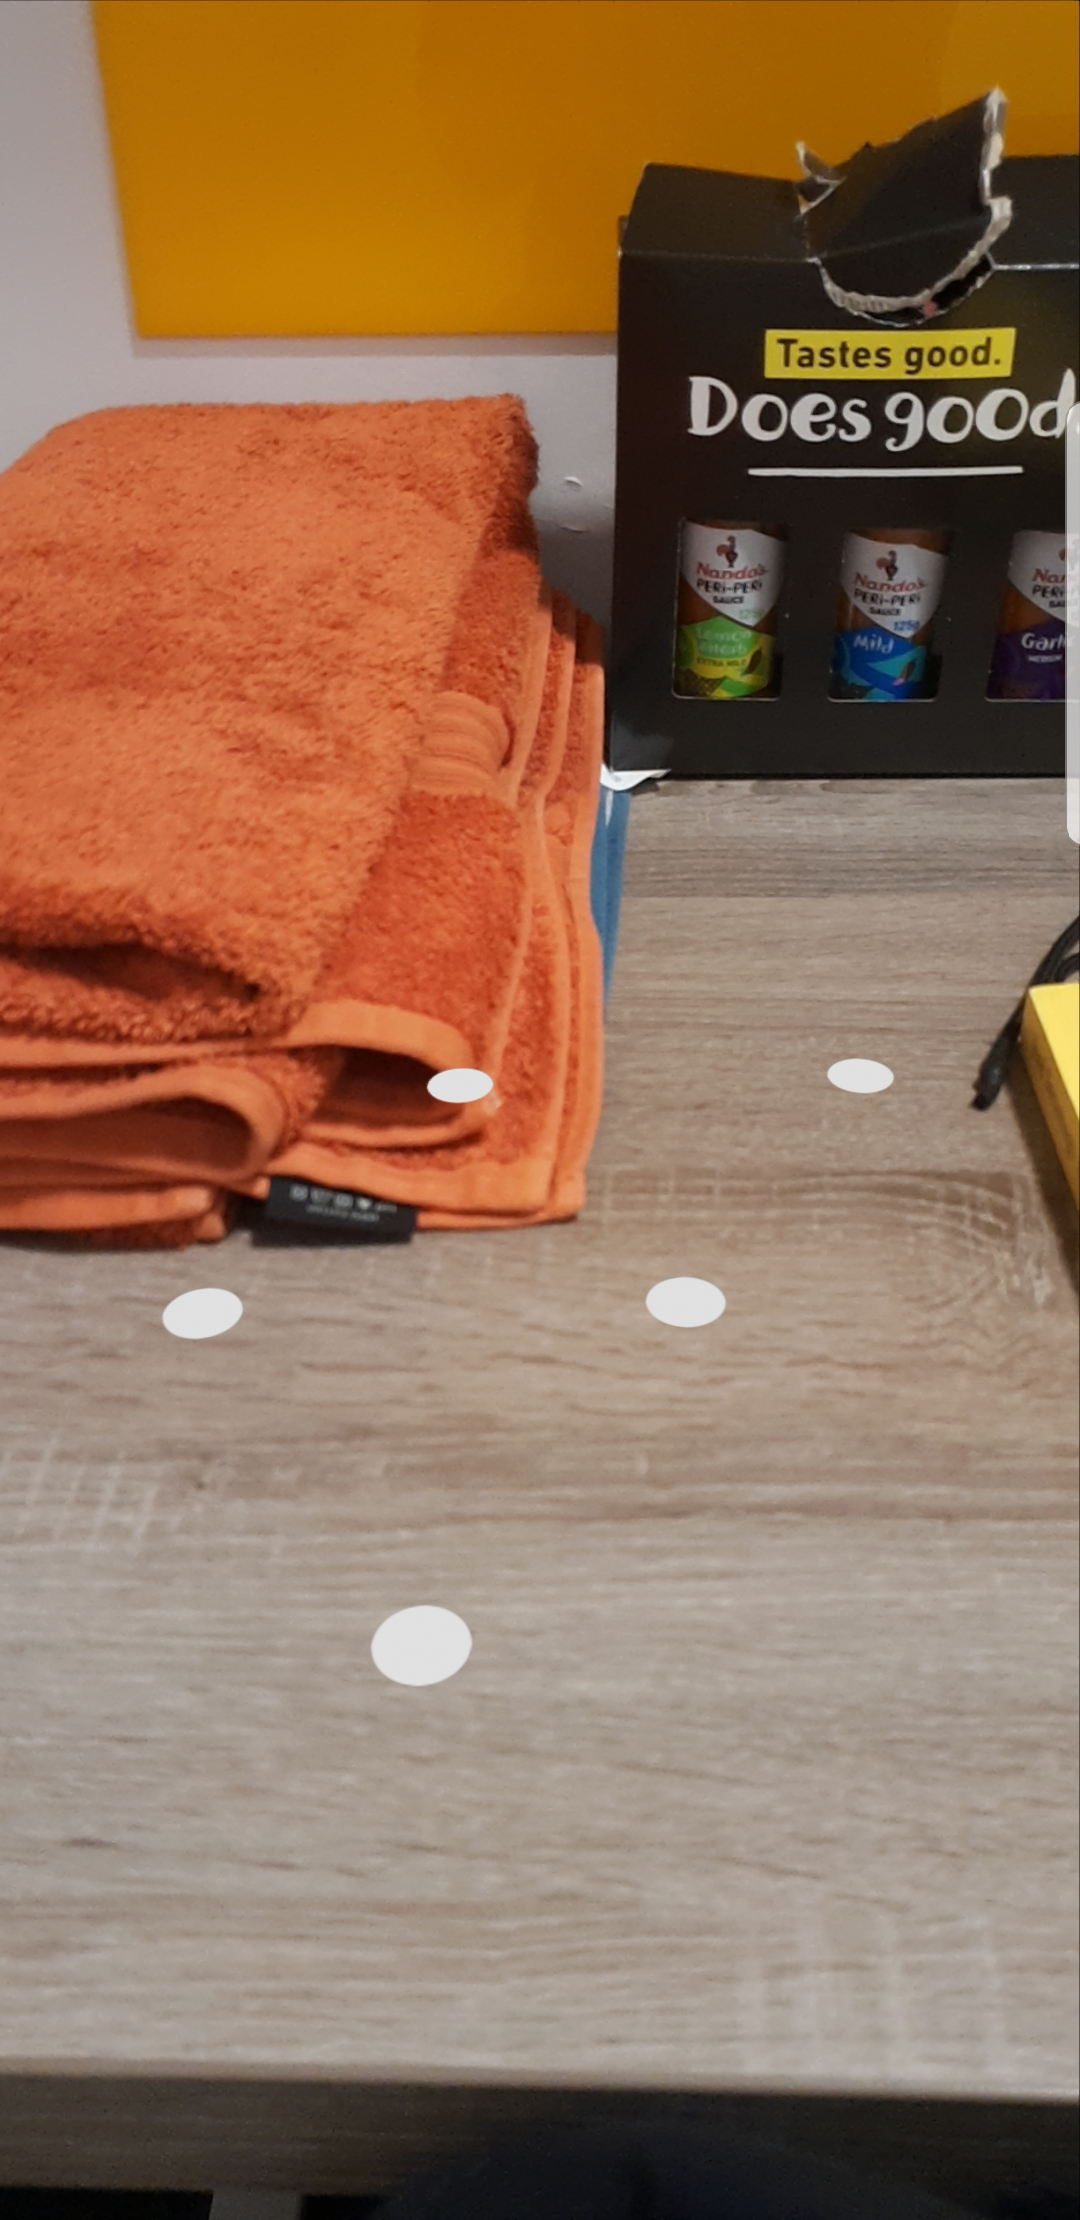
\includegraphics[width=60mm, height=100mm]{prototypes/ar/android/2.jpg} \\
(a) Initial view & (b) Detection of surface \\[6pt]
\multicolumn{2}{c}{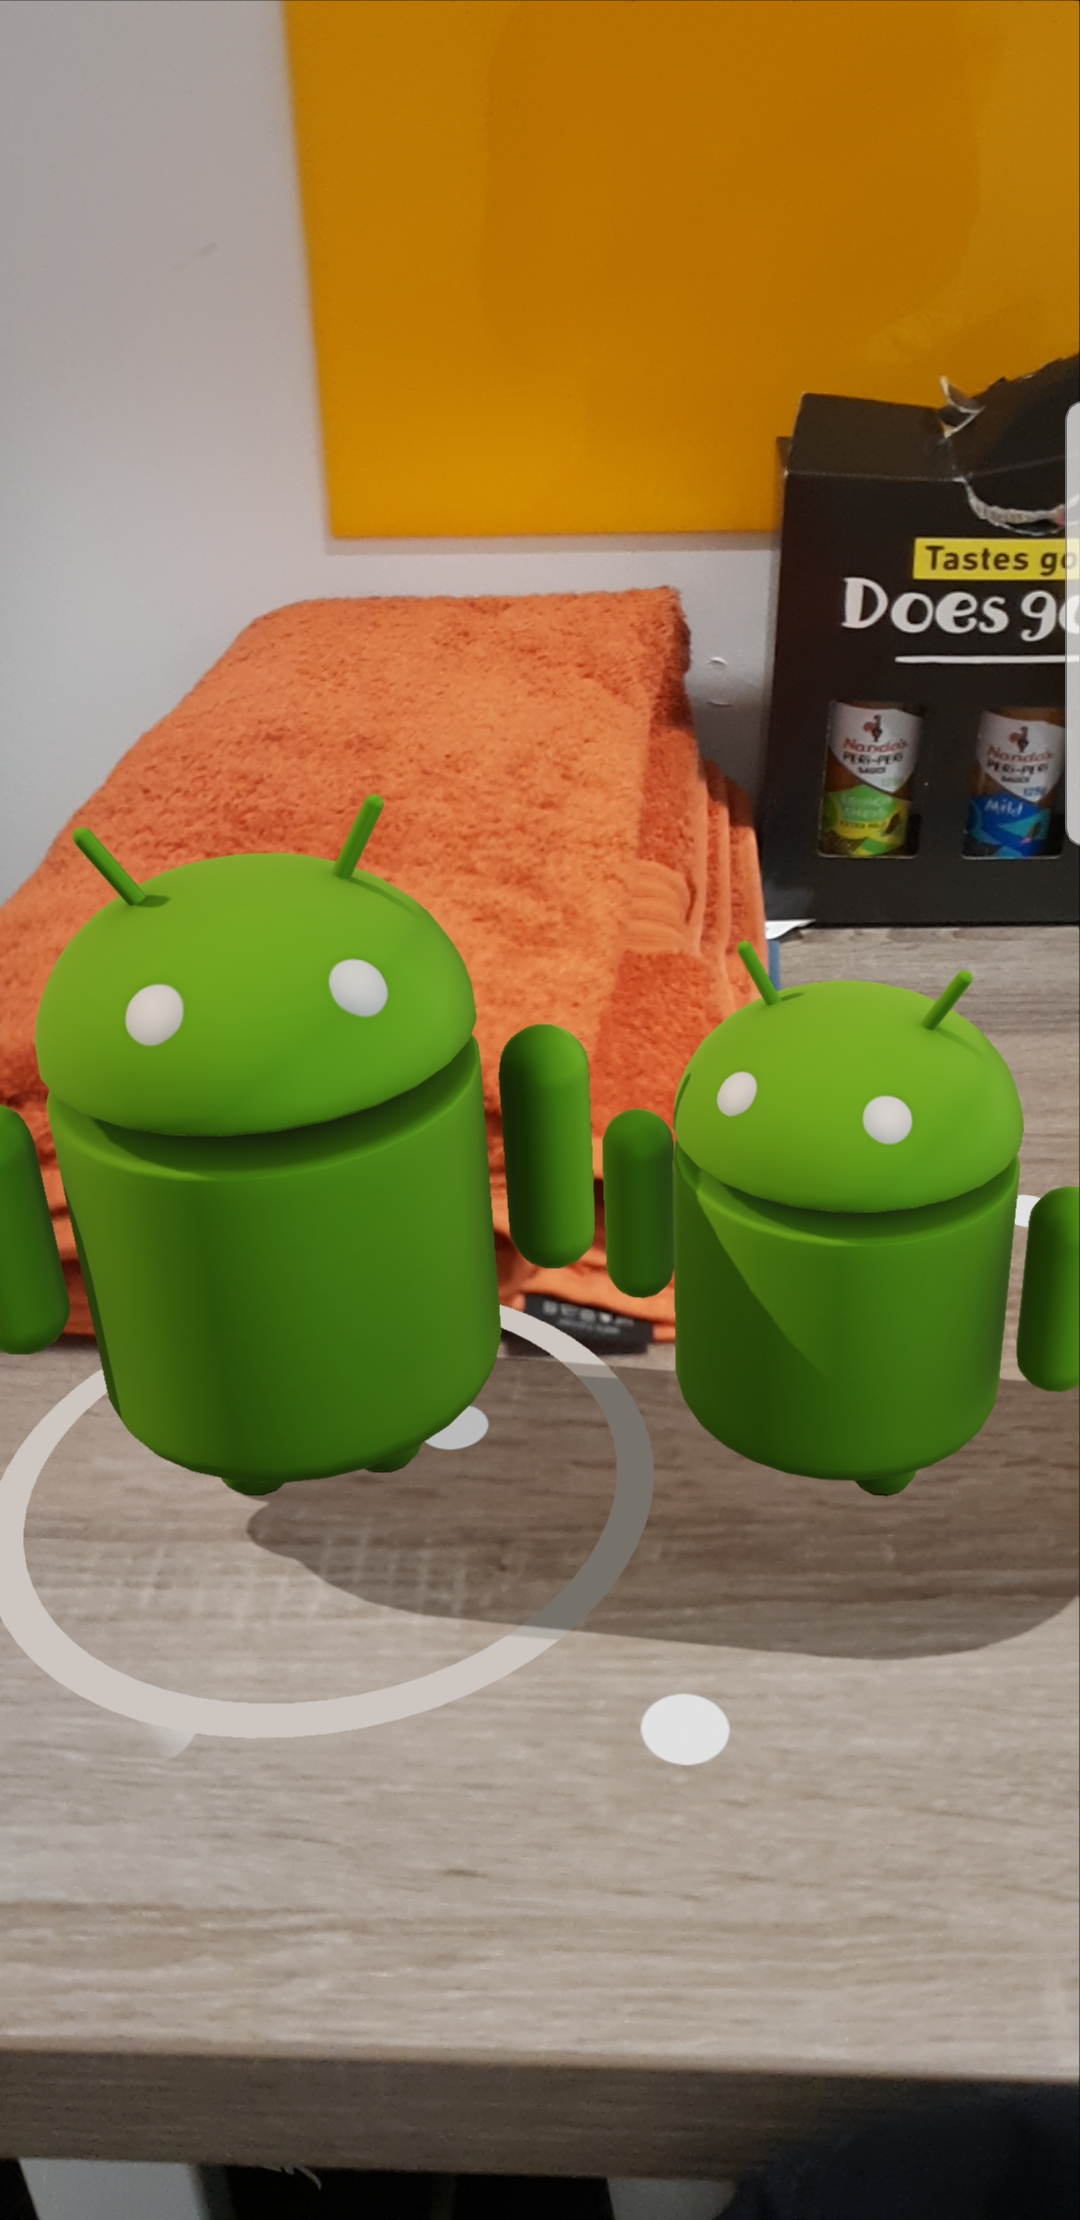
\includegraphics[width=60mm, height=100mm]{prototypes/ar/android/3.jpg} }\\
\multicolumn{2}{c}{(c) Objects superimposed on surface}
\end{tabular}
\caption{ARCore prototyping on Android device}
\label{fig:ARCore}
\end{figure}

\newpage
\subsubsection{Android Sensors Logging}
\begin{figure}[H]
    \centering
    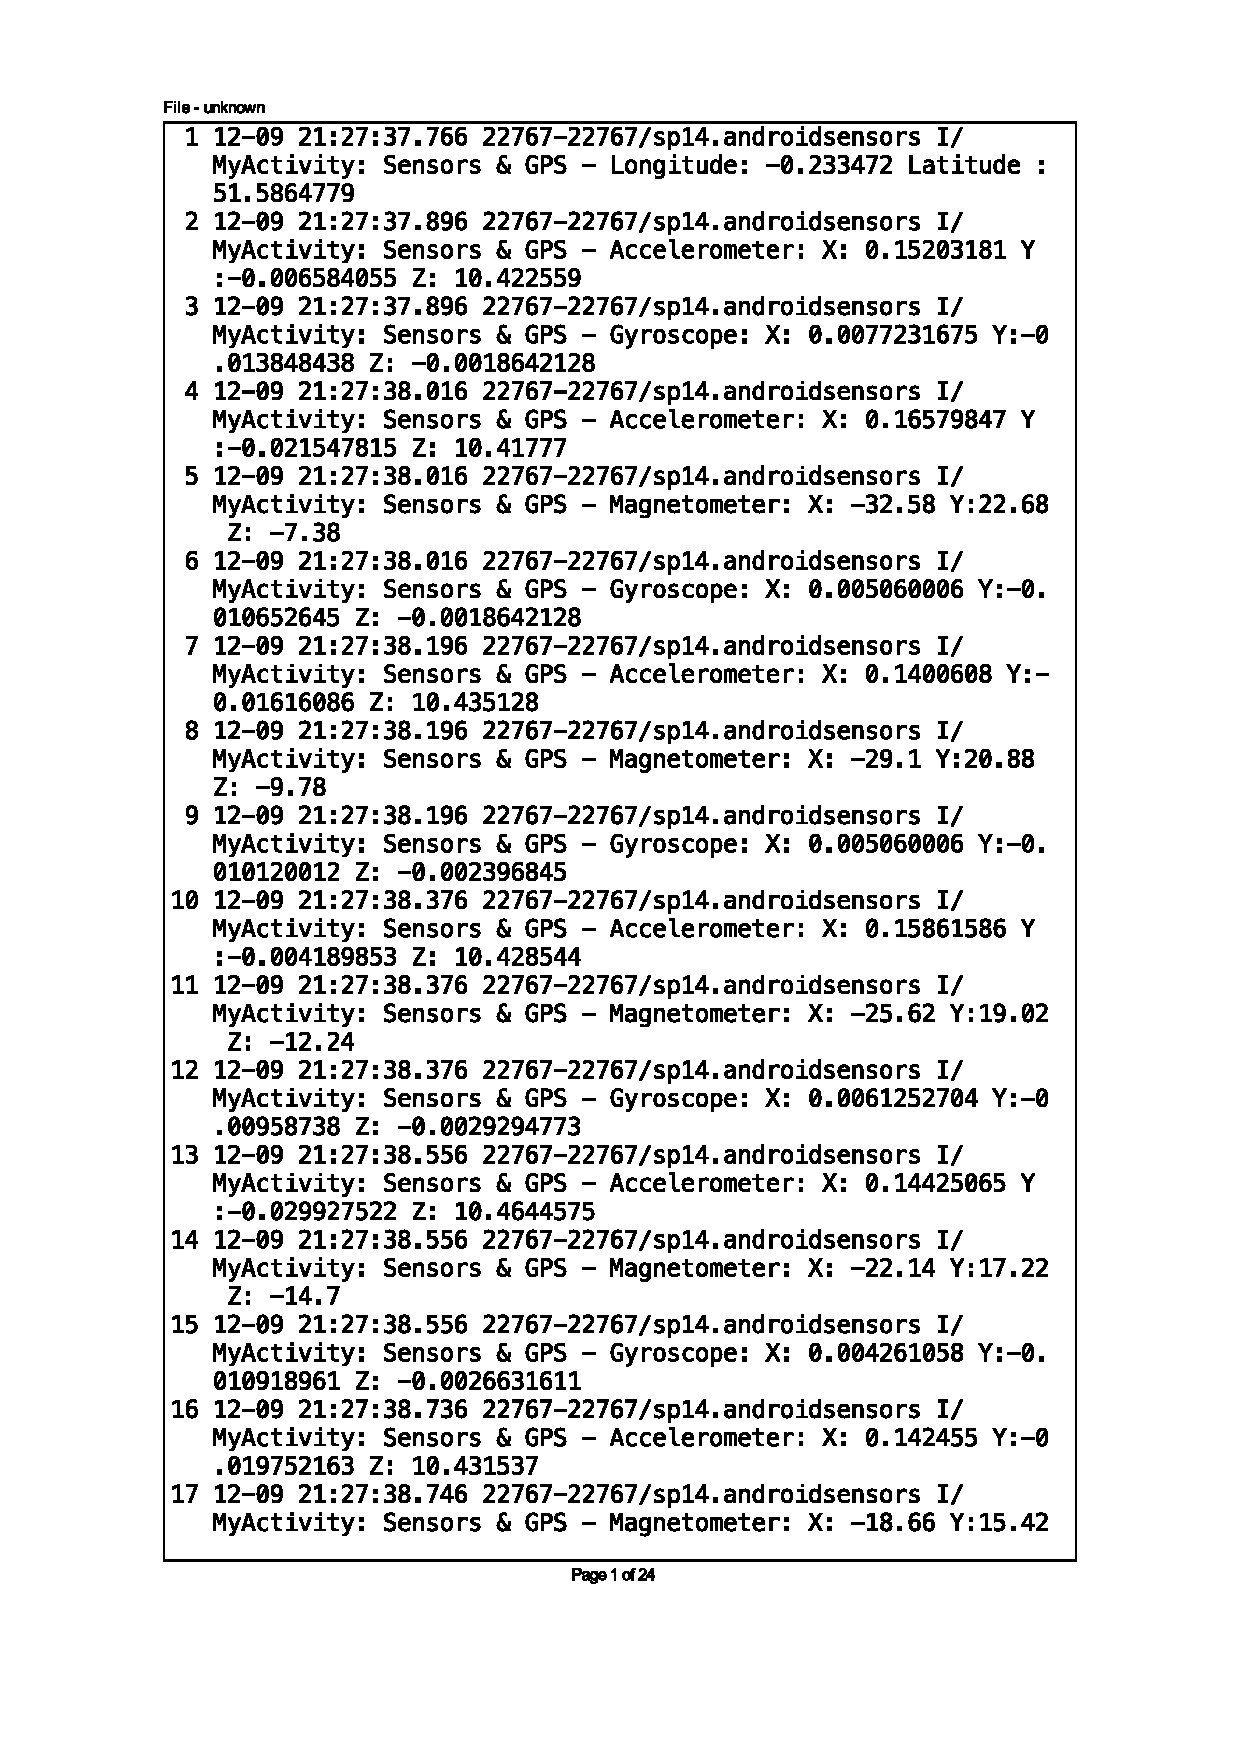
\includegraphics[width=\textwidth]
    {prototypes/ar/android/logs.pdf}
    \caption{GPS, accelerometer, magnometer, and gyroscope sensor data from an Android device over 1 second period}
    \label{fig:Android sensors logging}
\end{figure}

\subsection{UI/UX Prototypes}
\subsubsection{Storyboard}
\begin{figure}[H]
    \centering
    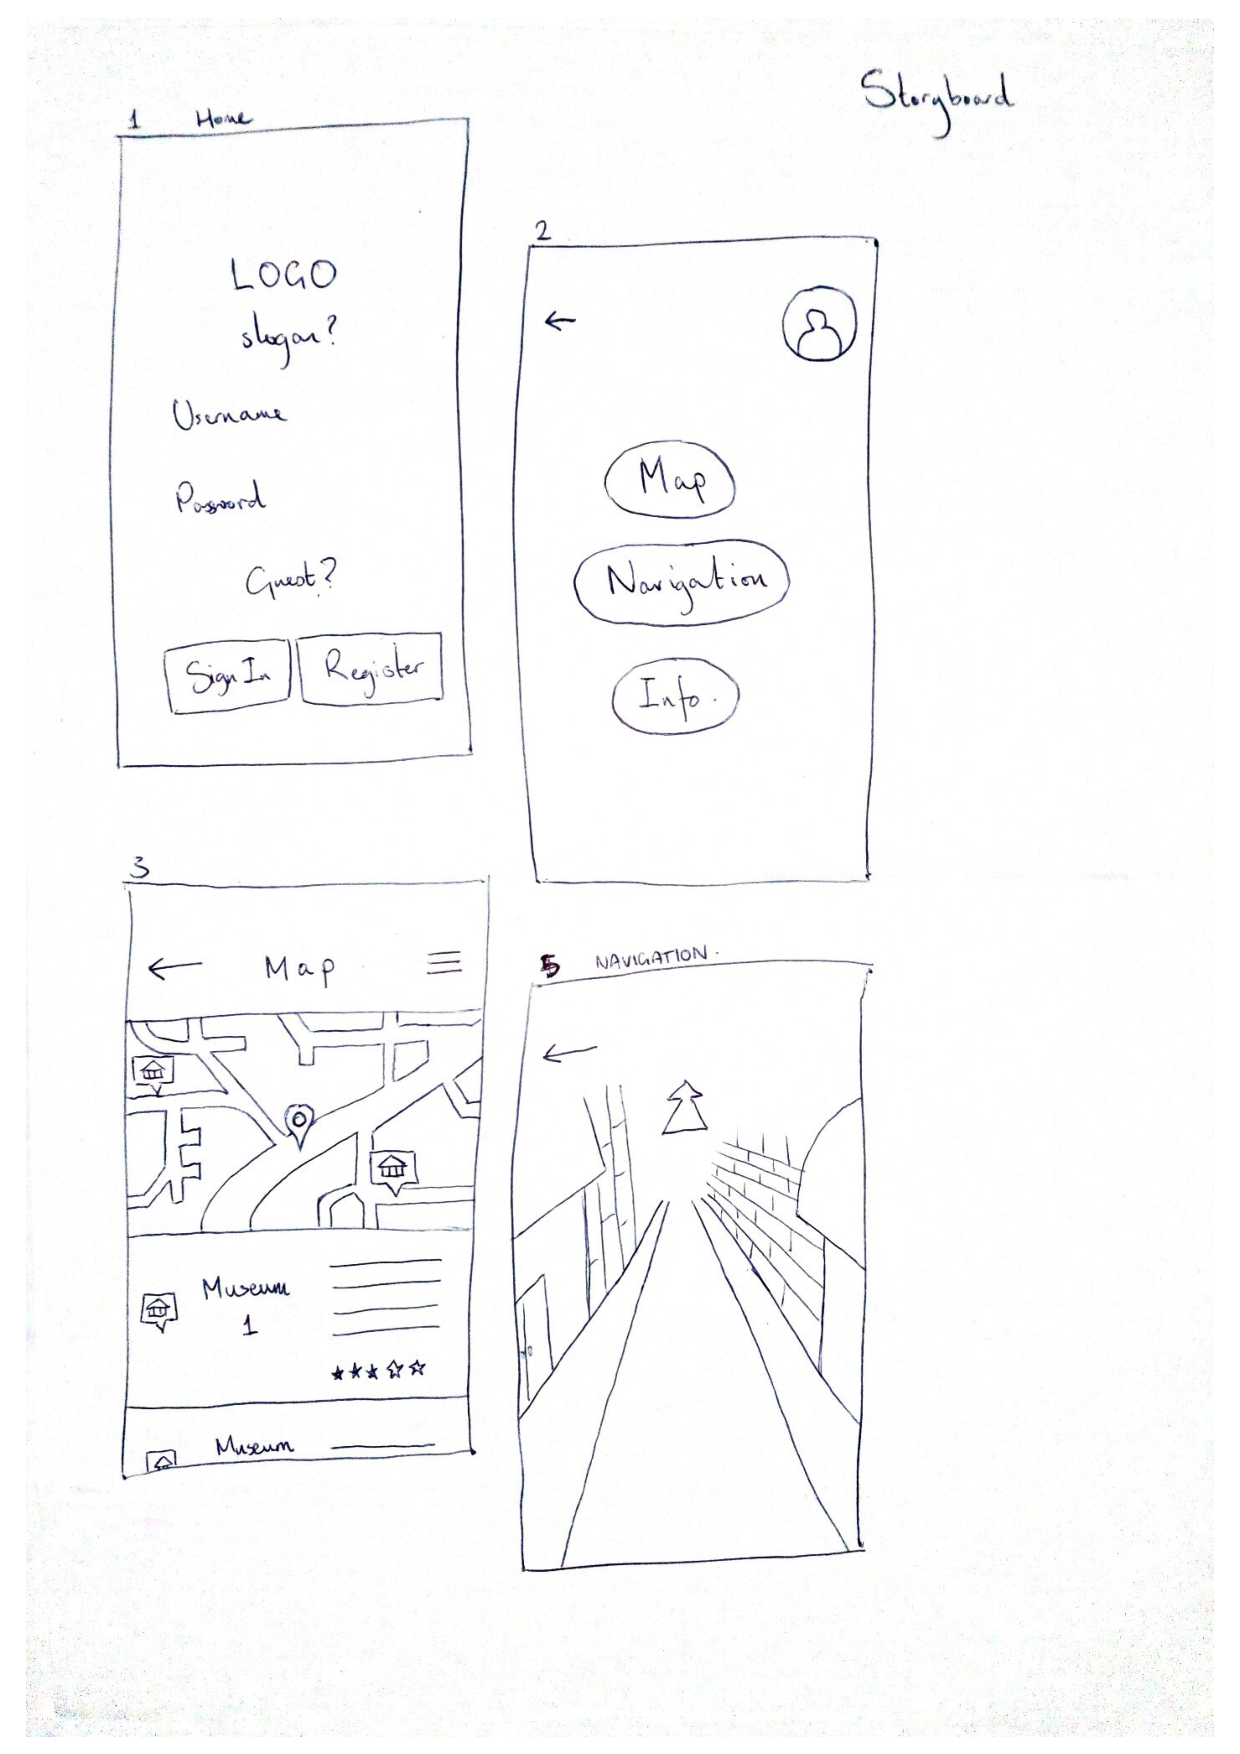
\includegraphics[width=\textwidth]
    {prototypes/ui/storyboard/1.pdf}
    \caption{Storyboard UI Drawings Page 1}
    \label{fig:storyboard}
\end{figure}

\newpage
\begin{figure}[H]
    \centering
    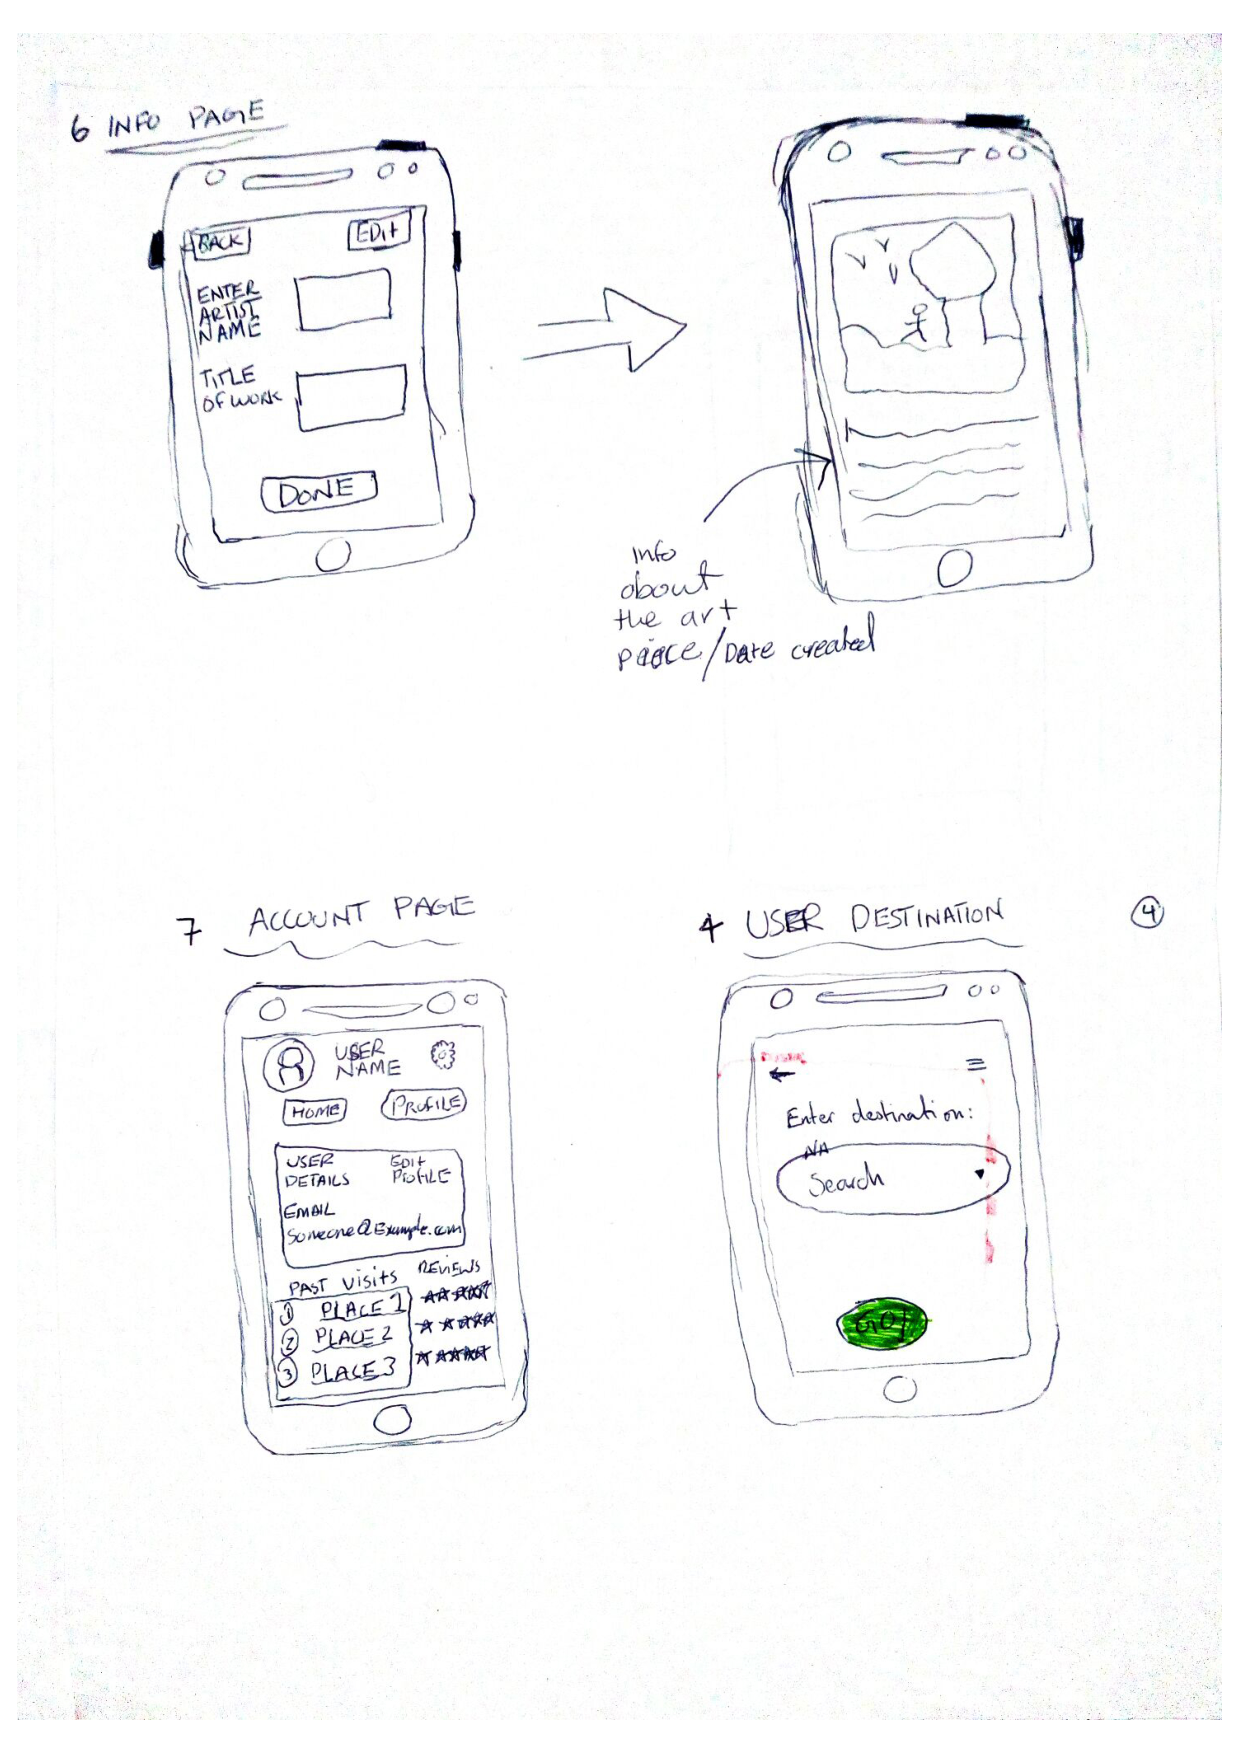
\includegraphics[width=\textwidth]
    {prototypes/ui/storyboard/2.pdf}
    \caption{Storyboard UI Drawings Page 1}
\end{figure}

\newpage
\begin{figure}[H]
    \centering
    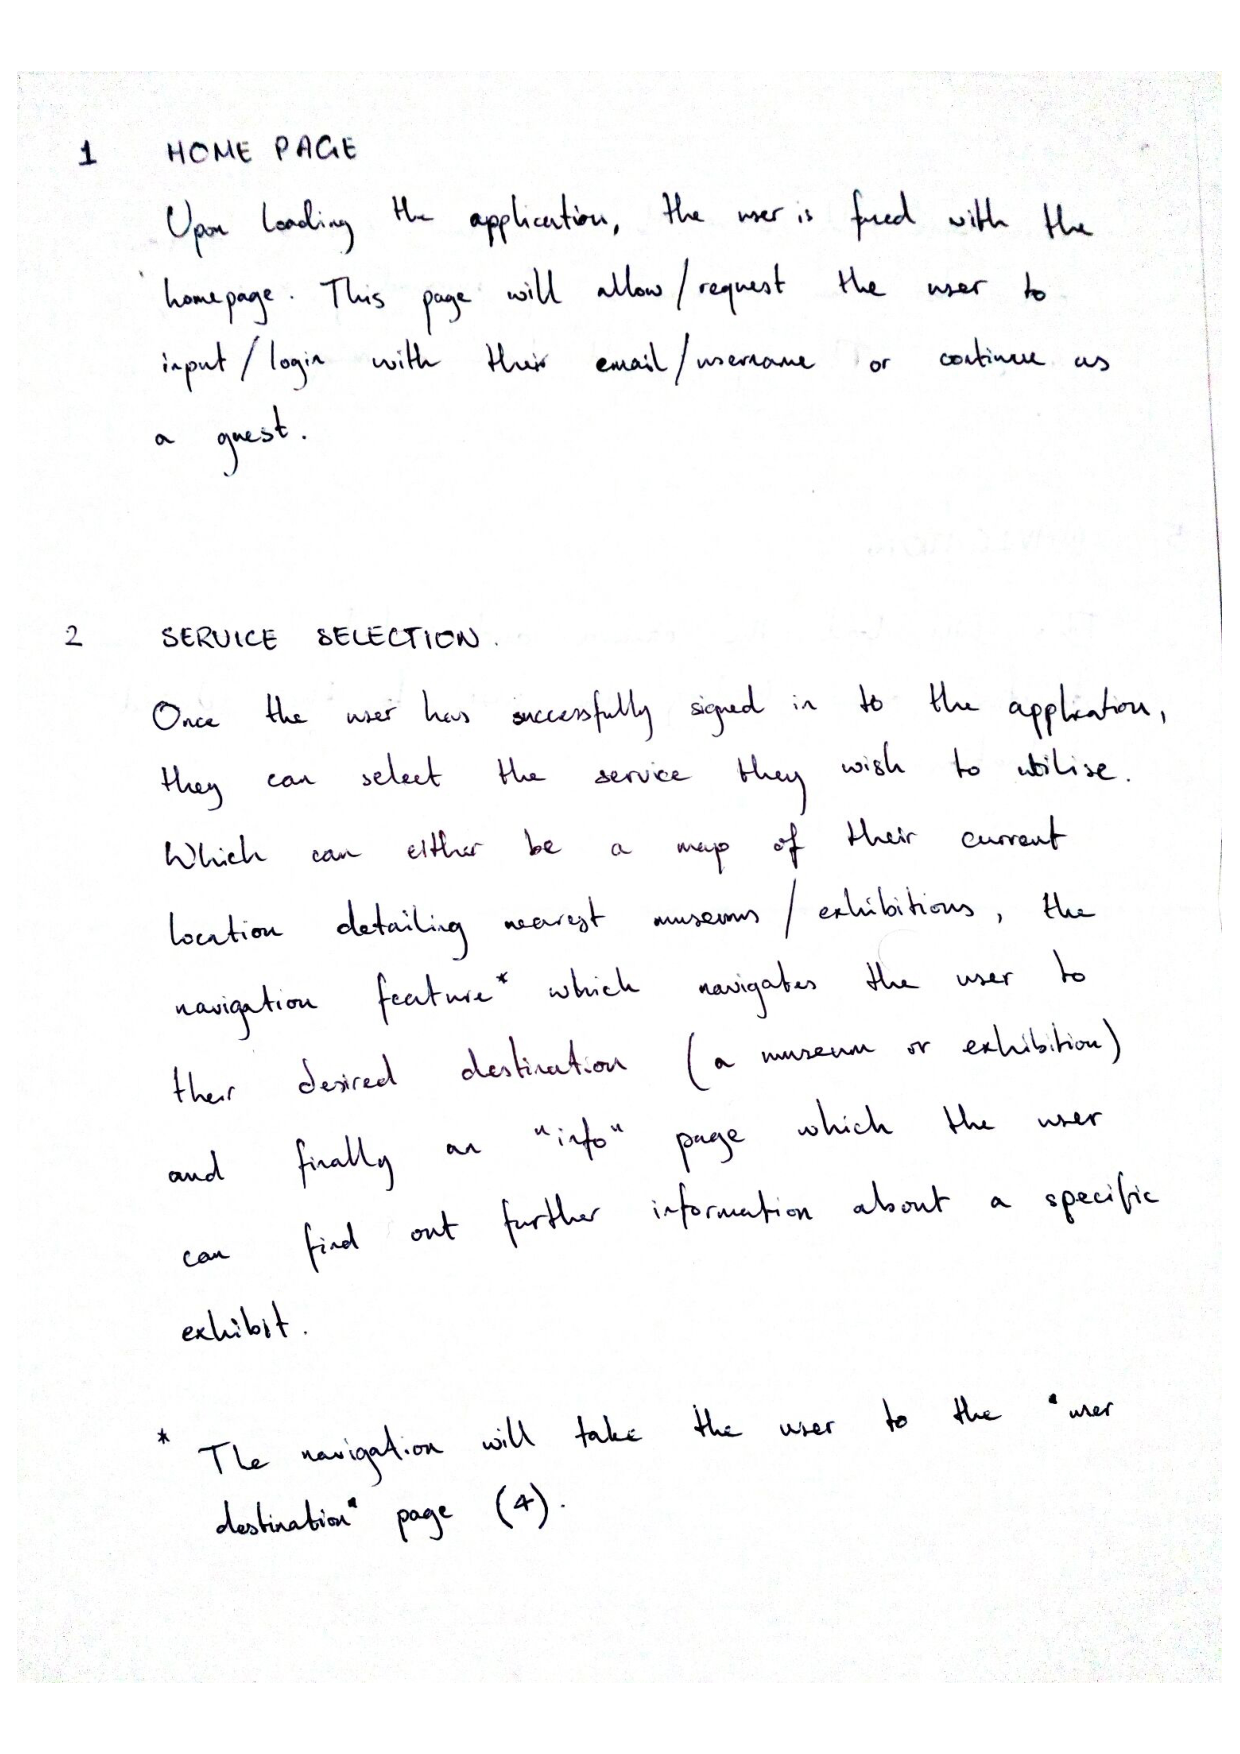
\includegraphics[width=\textwidth]
    {prototypes/ui/storyboard/3.pdf}
    \caption{Storyboard UI Descriptions Page 1}
\end{figure}

\newpage
\begin{figure}[H]
    \centering
    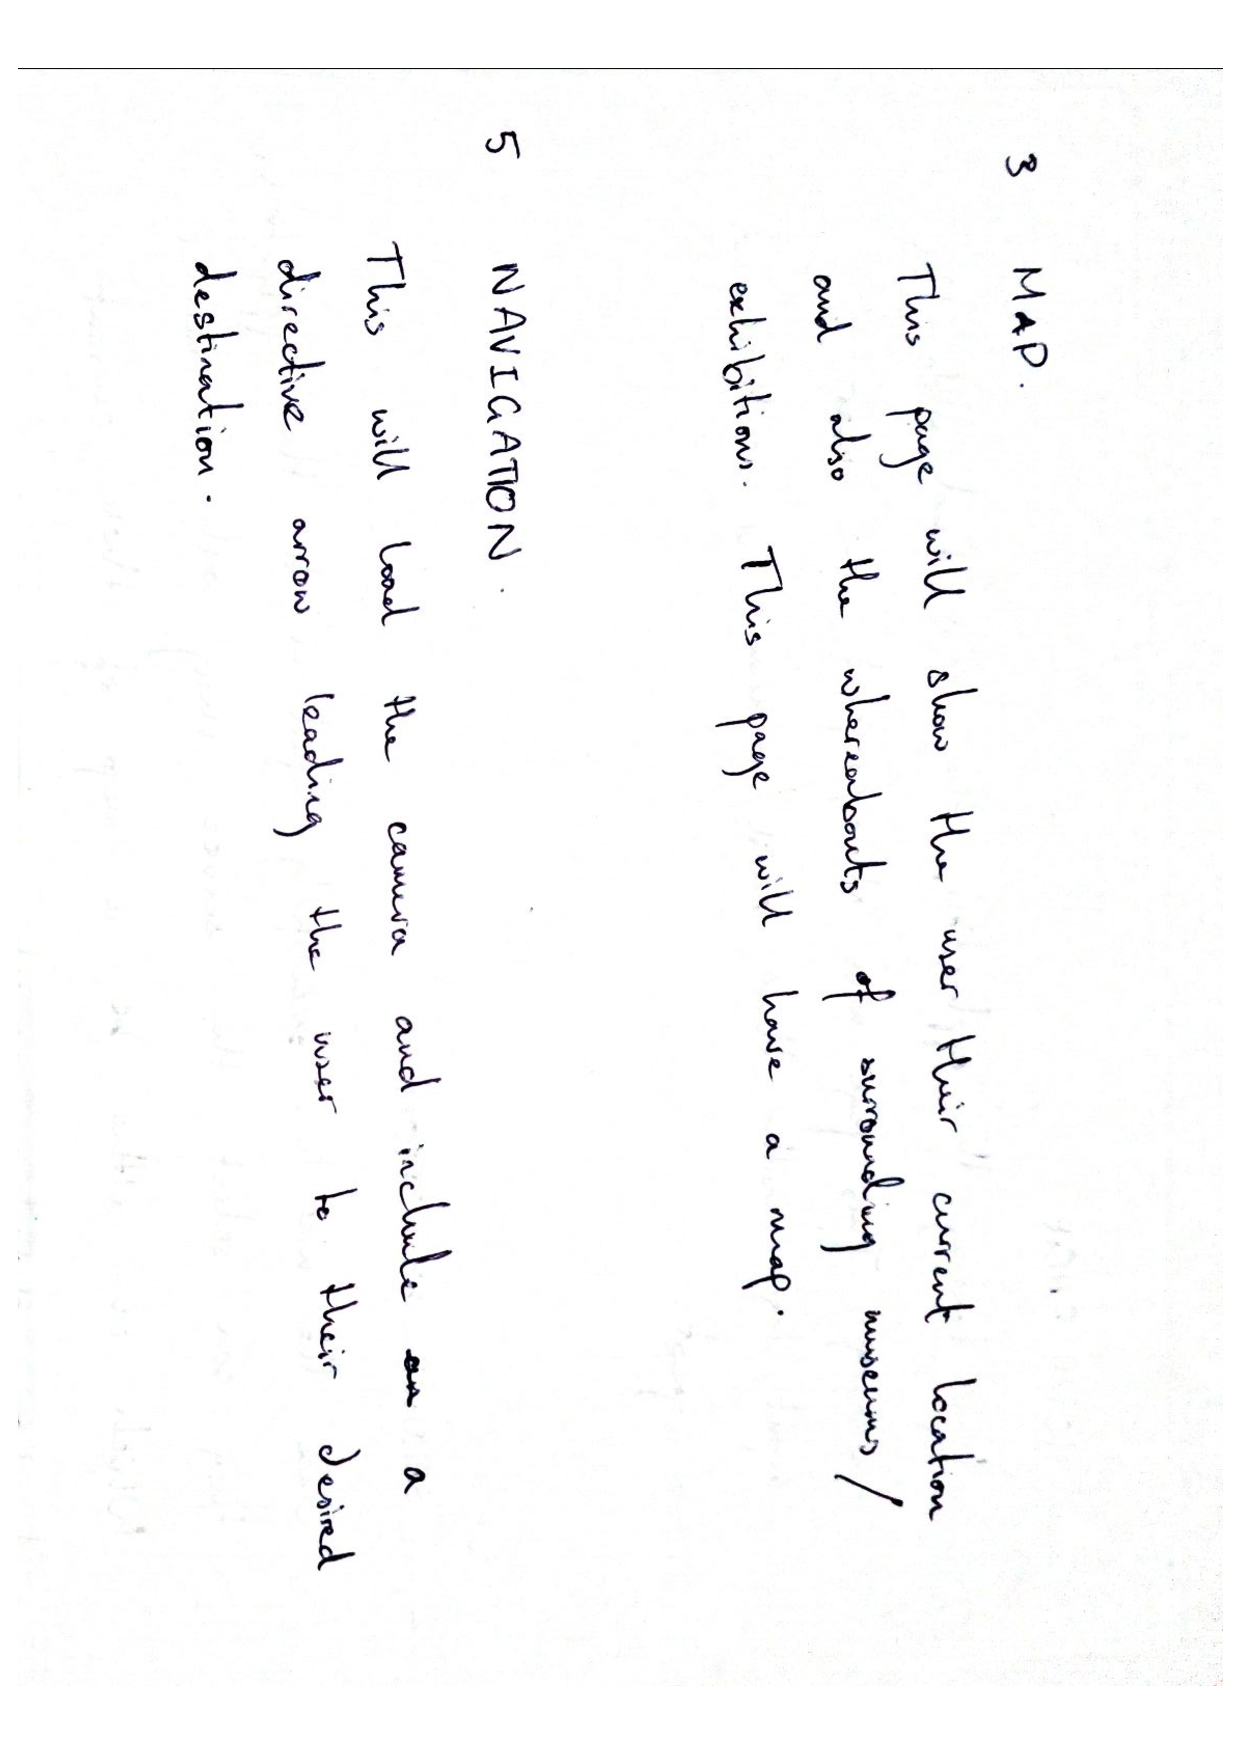
\includegraphics[angle=90, width=\textwidth]
    {prototypes/ui/storyboard/4.pdf}
    \caption{Storyboard UI Descriptions Page 2}
\end{figure}

\newpage
\begin{figure}[H]
    \centering
    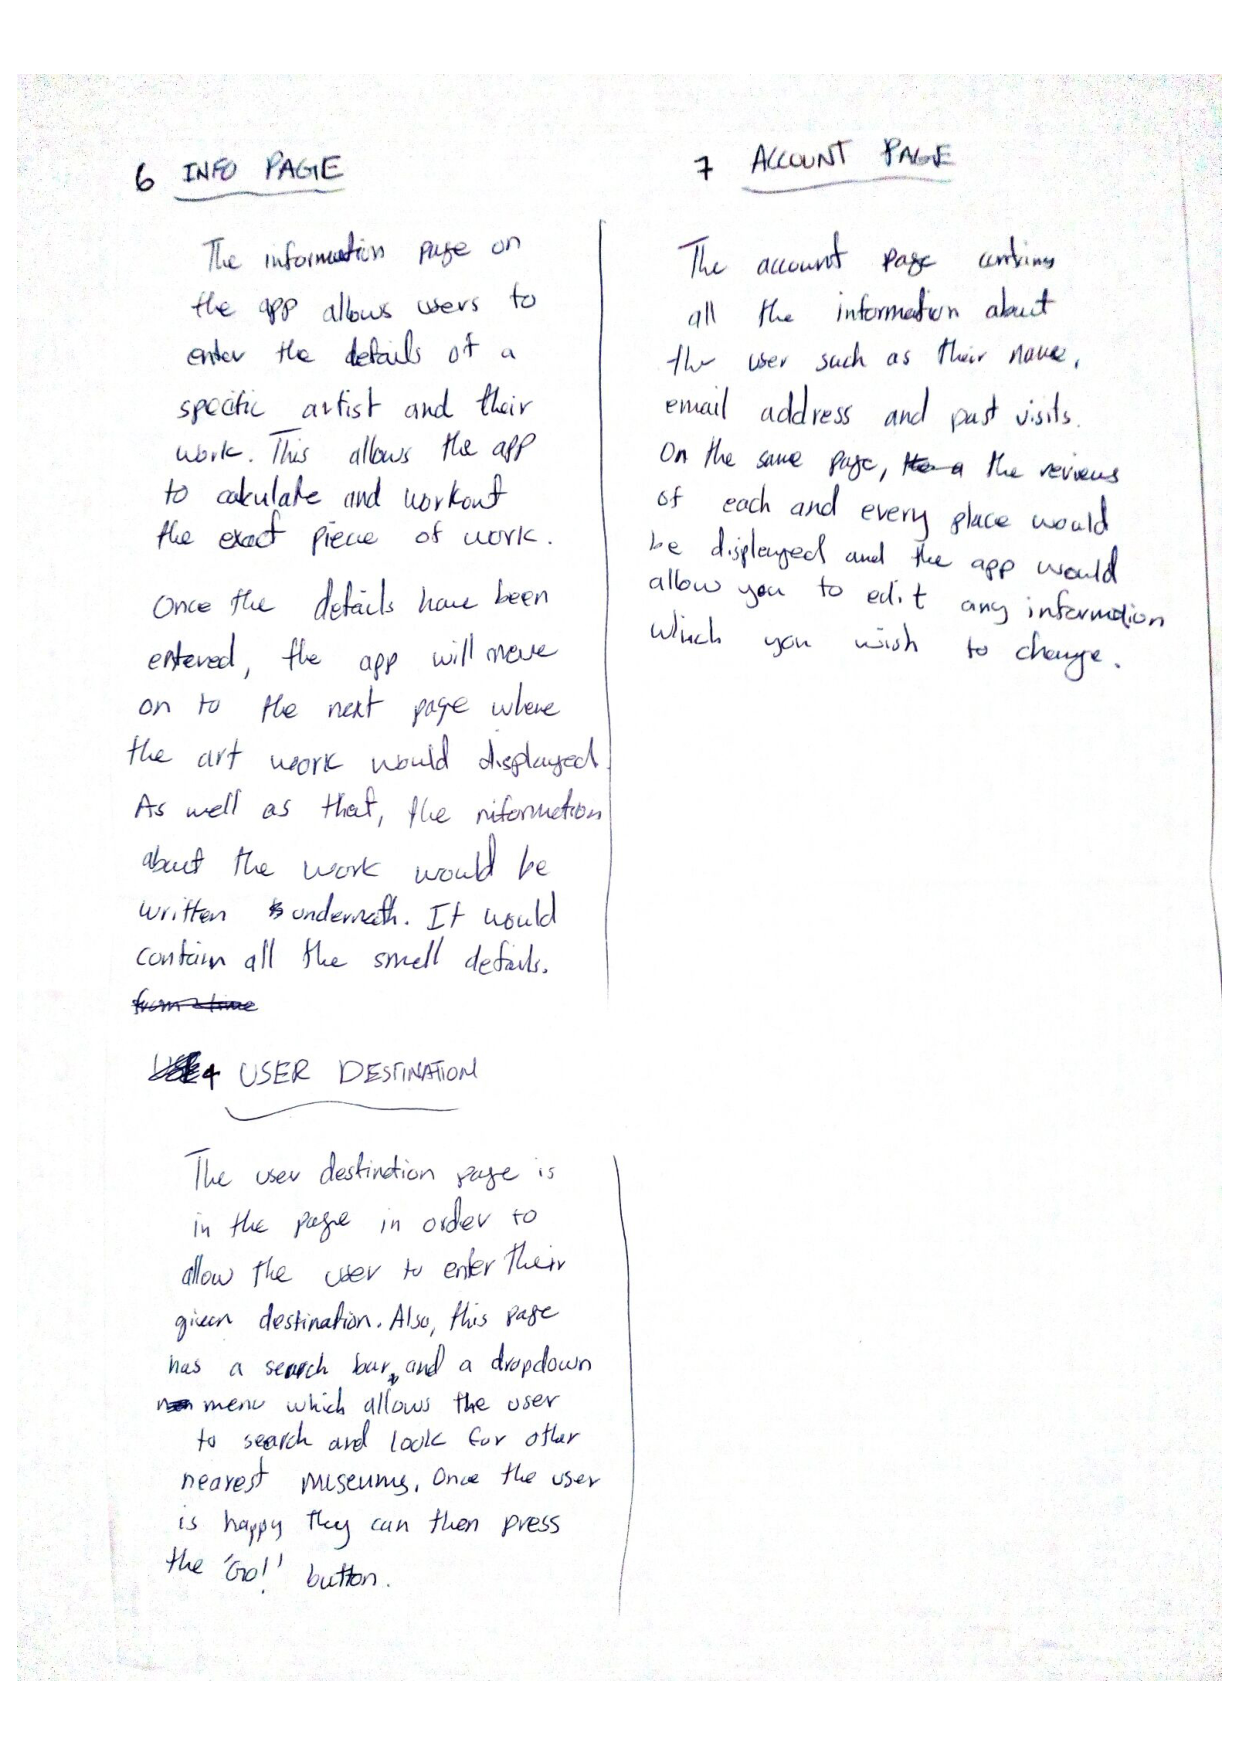
\includegraphics[width=\textwidth]
    {prototypes/ui/storyboard/5.pdf}
    \caption{Storyboard UI Descriptions Page 3}
\end{figure}

\subsubsection{Prototype 1}
\begin{figure}[H]
    \centering
    \includegraphics[width=\textwidth]
    {prototypes/ui/1.png}
    \caption{Overview of UI Prototype 1}
    \label{fig:prototype1}
\end{figure}

\subsubsection{Prototype 2}
\begin{figure}[H]
    \centering
    \includegraphics[width=\textwidth]
    {prototypes/ui/2.png}
    \caption{Overview of UI Prototype 2}
    \label{fig:prototype2}
\end{figure}

\subsubsection{Prototype 3}
\begin{figure}[H]
    \centering
    \includegraphics[width=\textwidth]
    {prototypes/ui/3.png}
    \caption{Overview of UI Prototype 3}
    \label{fig:prototype3}
\end{figure}

\newpage
\subsubsection{Prototype Reviews}
\textbf{Prototype 1}\\
This prototype again is very plain but this is made to look it as it looks more professional and although the prototype has a lot of buttons, this greatly considers the end user and what things we would want to do on the application making the potential of it greater. The search function and the map feature makes it a lot more personal to the user with potential options that they may select. Overall, because it considers the user more, this type of format at least should be used in the final version. One suggestion would be to maybe include colour as well as improve the logo because it is not very clear what the application is from looking at this, so have a logo to reflect this. The separate page for the use of AR is very good but one concern is how the the app will detect will where the user is or whether they can use the AR feature anywhere even without visiting the museum.\\

\textbf{Prototype 2}\\
The prototype at first glance looks very plain and with not much information or scope for the user to explore the app and seems very limited. One of the key things which could improve the app is simply to add colour to make it more appealing and engaging to users. Also, it is not very clear what the application is used for and how it can improve the existing method of visiting a museum - which I now know what the app’s purpose is - where a visitor can just have a guided tour from an expert or even an auditory tour. Certain features of the prototype were good such as the search feature and the clarity making the app user-friendly. As well as this, the fact that the app shows the closest museum to the input given is very helpful, showing the rating given by visitors making easier to choose which museum to visit. The fact that it also has logout confirmation page and a page showing the users account where they can add favourite museums and add ratings and reviews gives other users better choice where they can make a more informed decision.\\

\textbf{Prototype 3}\\
The prototype is quite plain at first glance although the use of colour through the background is good. It is more appealing and engaging. However, use of the application seems very basic and limited with little function. The prototype consists mainly of buttons and doesn’t allow much user input, that being said, the search function is a good addition. Overall, this prototype is very limited and use of the prototype 2 should be used over this one.

\newpage
\subsubsection{Final Prototype}
\begin{figure}[H]
    \centering
    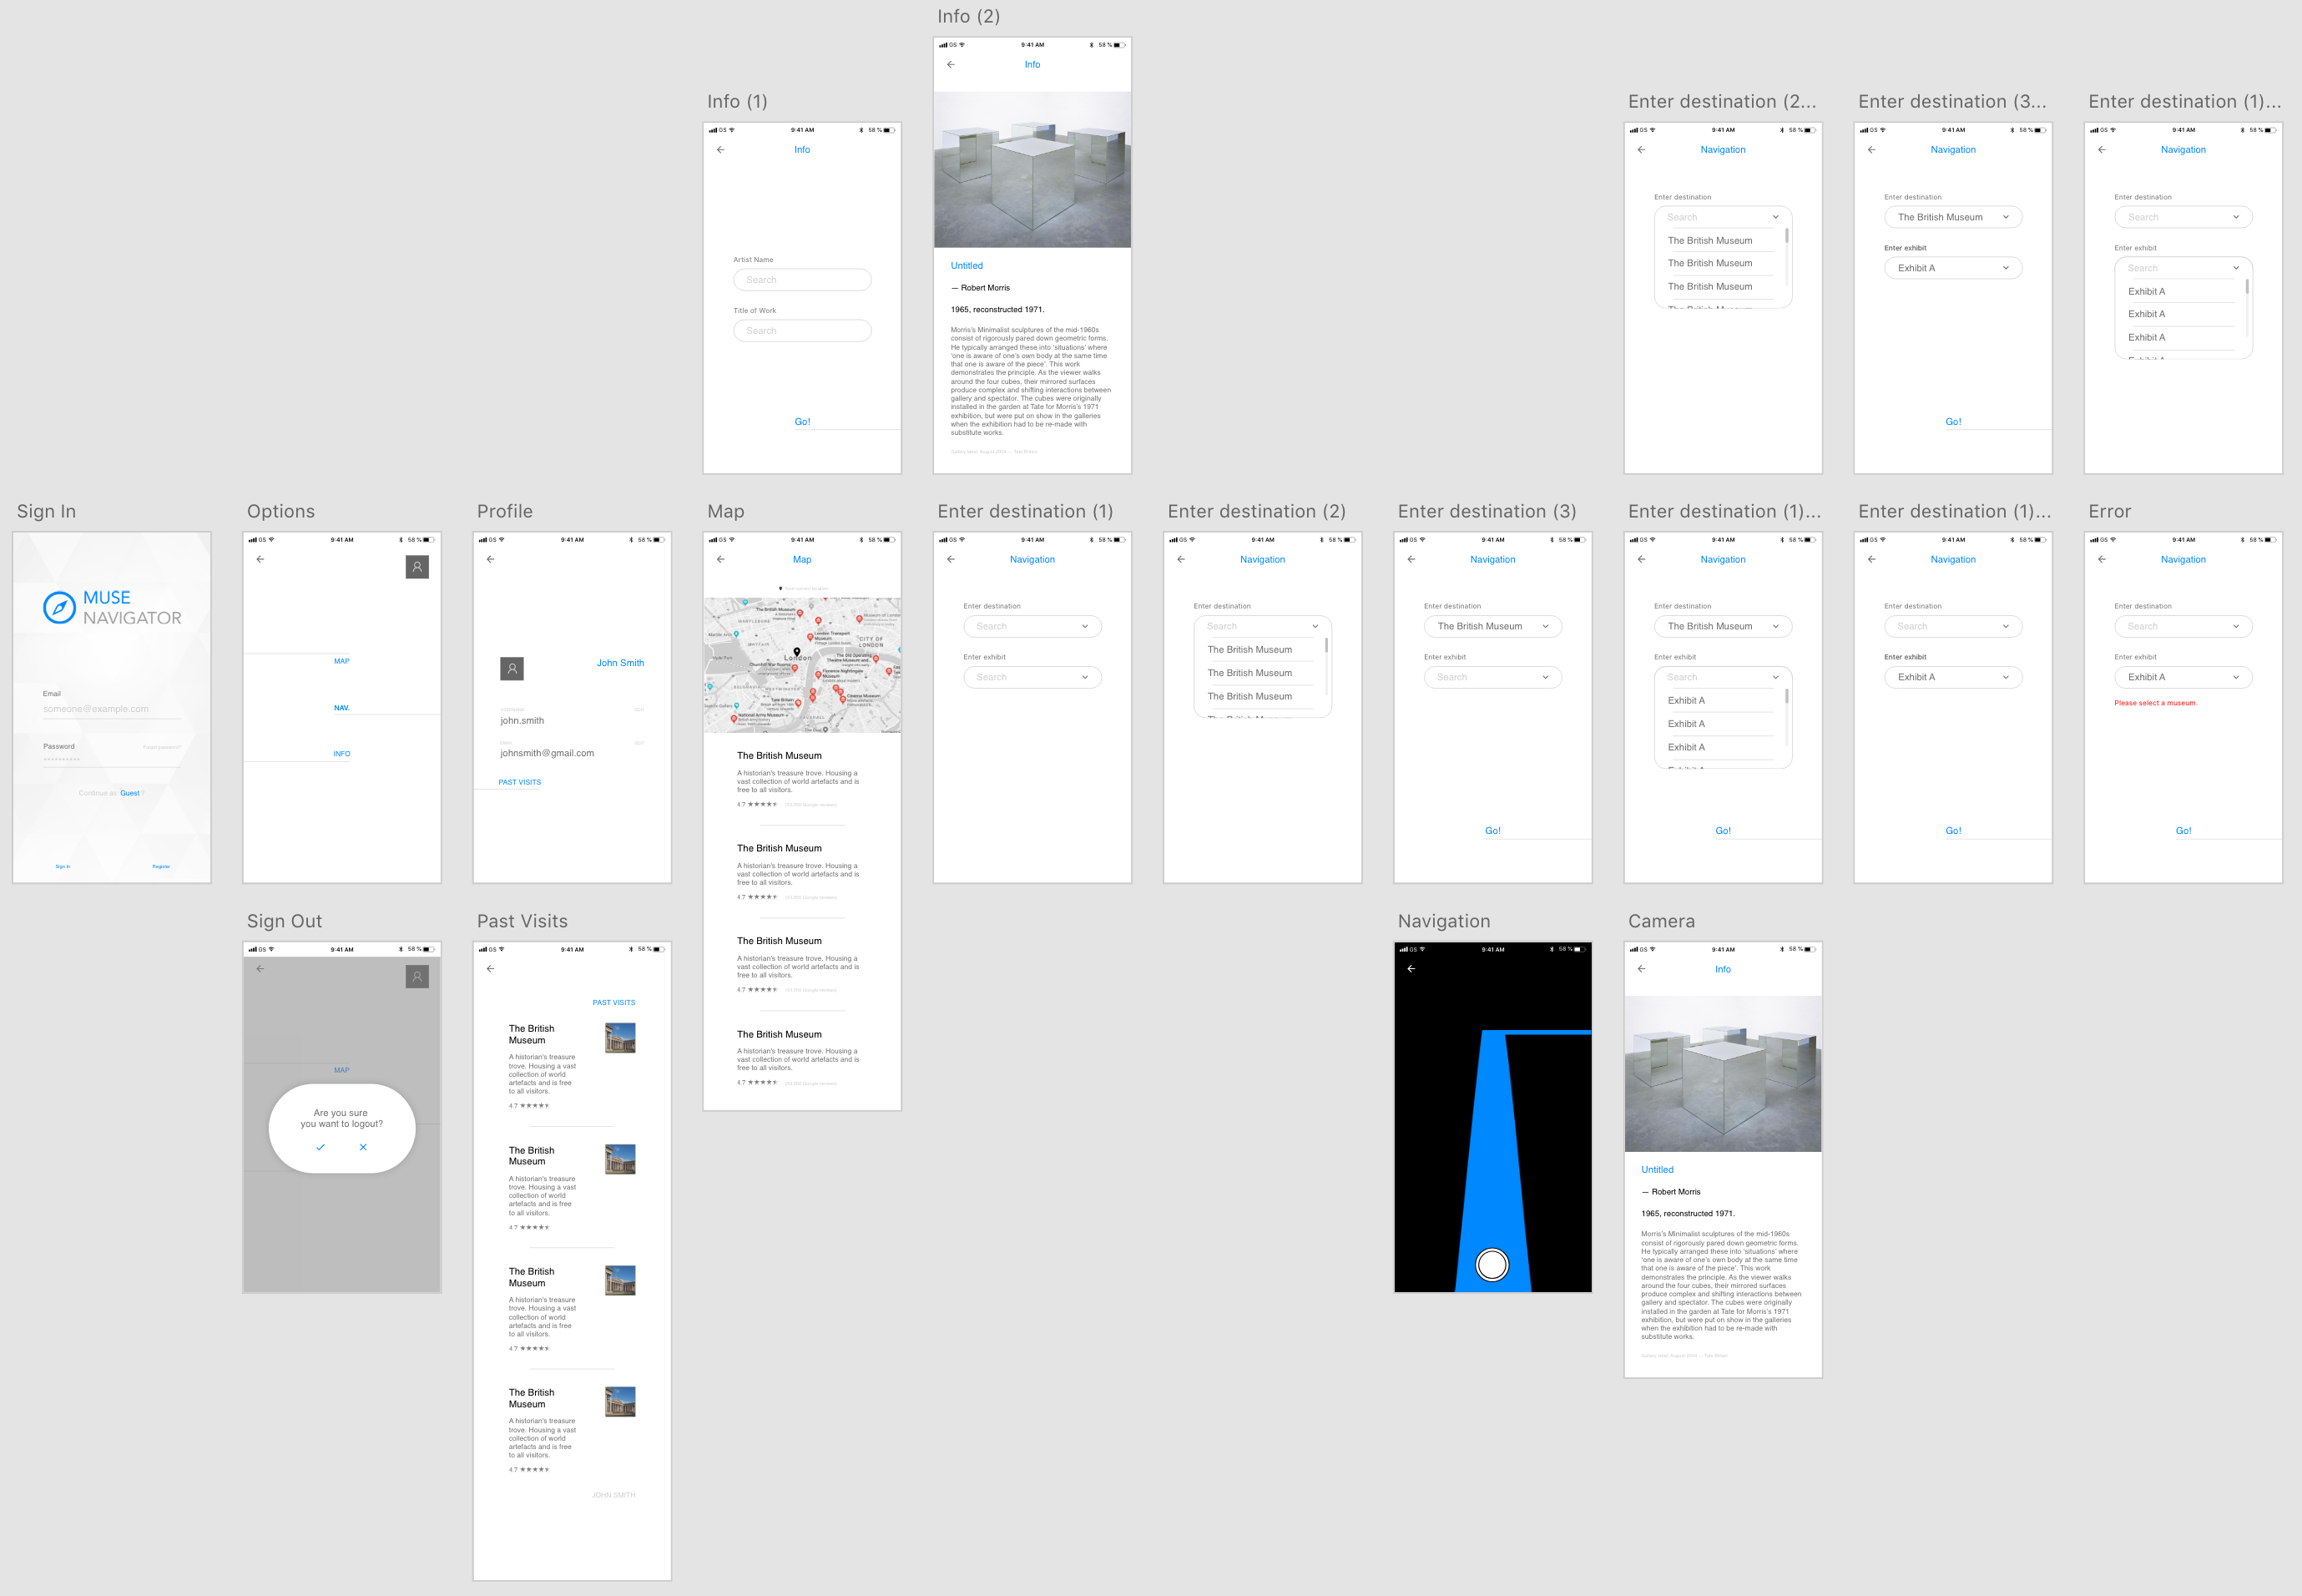
\includegraphics[angle=90, width=\textwidth]
    {prototypes/ui/final.png}
    \caption{Overview of final UI prototype}
    \label{fig:finaloverview}
\end{figure}

\newpage
\begin{figure}[H]
\centering
\begin{tabular}{cc}
  \includegraphics[width=60mm, height=100mm]{prototypes/ui/final/1.png} &   \includegraphics[width=60mm, height=100mm]{prototypes/ui/final/2.png} \\
(a) Sign in  & (b) Options \\[6pt]
 \includegraphics[width=60mm, height=100mm]{prototypes/ui/final/3.png} &   
\includegraphics[width=60mm, height=100mm]{prototypes/ui/final/4.png} \\
(c) Profile & (d) Past visits \\[6pt]
\end{tabular}
\caption{Final UI Designs of App}
\end{figure}

\newpage
\begin{figure}[H]
\centering
\begin{tabular}{cc}
  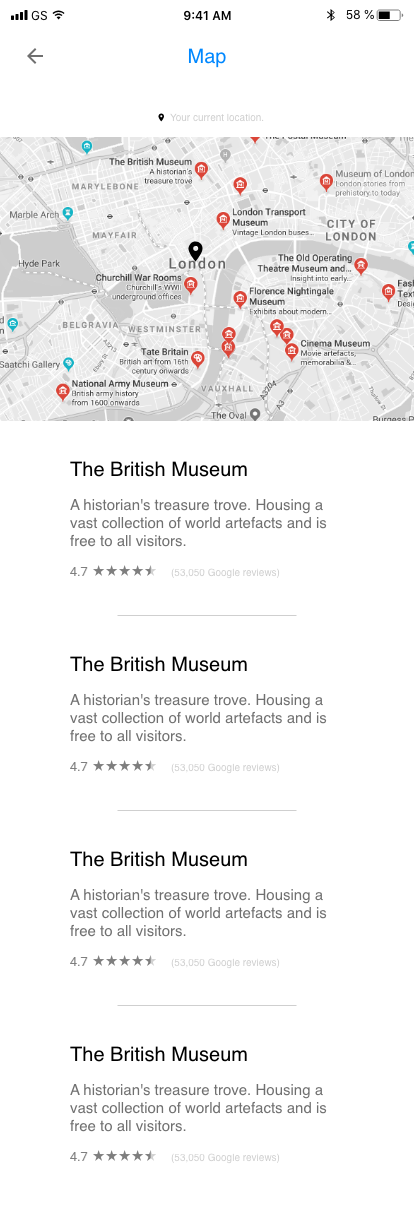
\includegraphics[width=60mm, height=100mm]{prototypes/ui/final/5.png} &   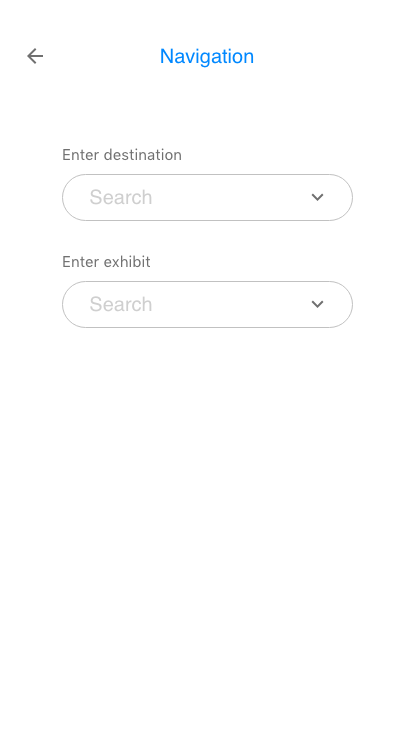
\includegraphics[width=60mm, height=100mm]{prototypes/ui/final/6a.png} \\
(e) Map of museums & (f) Destination \\[6pt]
 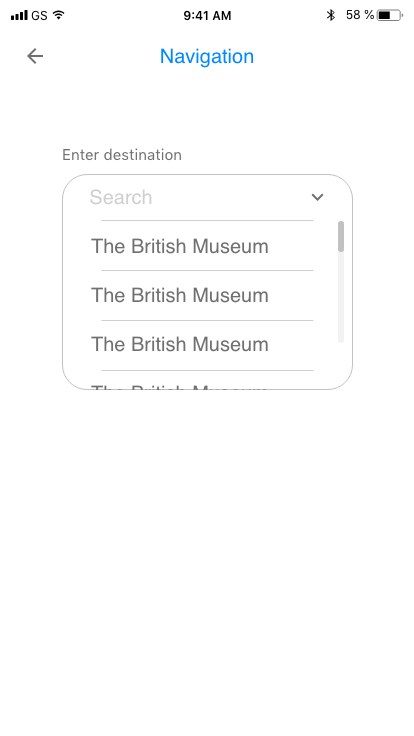
\includegraphics[width=60mm, height=100mm]{prototypes/ui/final/6b.png} &   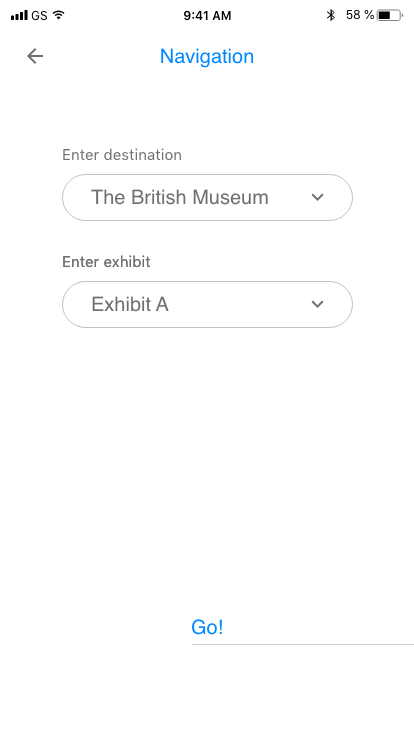
\includegraphics[width=60mm, height=100mm]{prototypes/ui/final/6c.png} \\
(g) Destination Dropdown & (h) Filled  \\[6pt]
\end{tabular}
\end{figure}

\newpage
\begin{figure}[H]
\centering
\begin{tabular}{cc}
  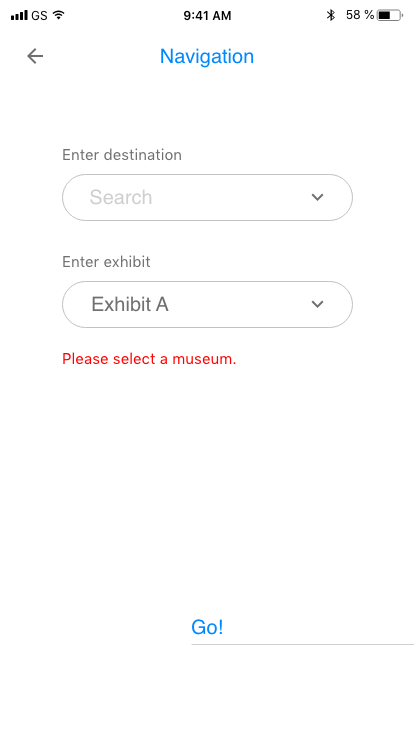
\includegraphics[width=60mm, height=100mm]{prototypes/ui/final/6d.png} &   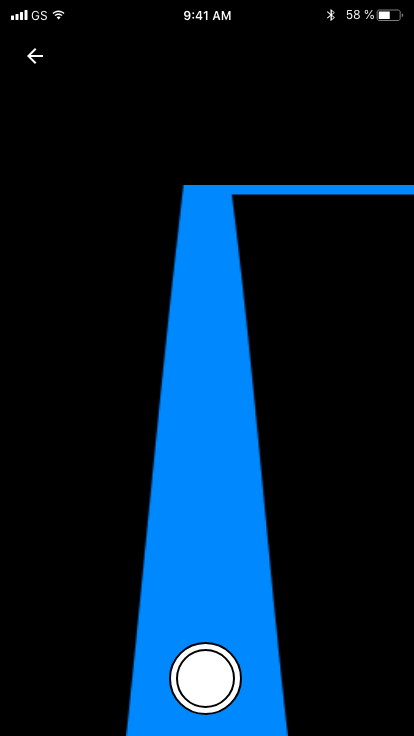
\includegraphics[width=60mm, height=100mm]{prototypes/ui/final/7.png} \\
(i) Error message & (j) AR Navigation \\[6pt]
 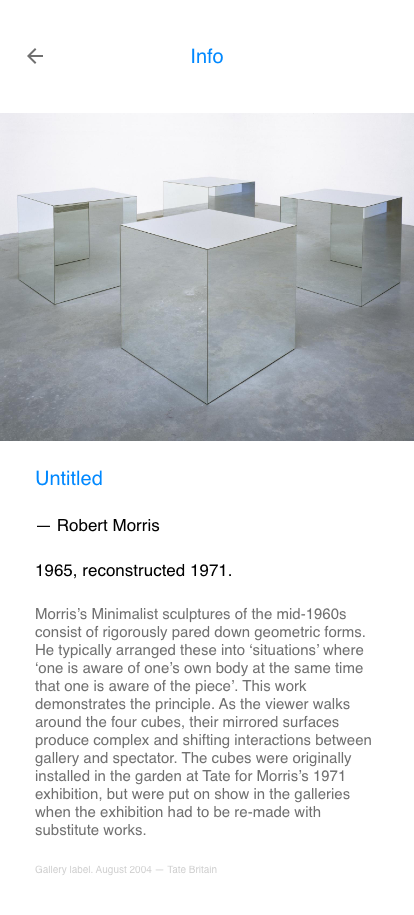
\includegraphics[width=60mm, height=100mm]{prototypes/ui/final/8.png} &   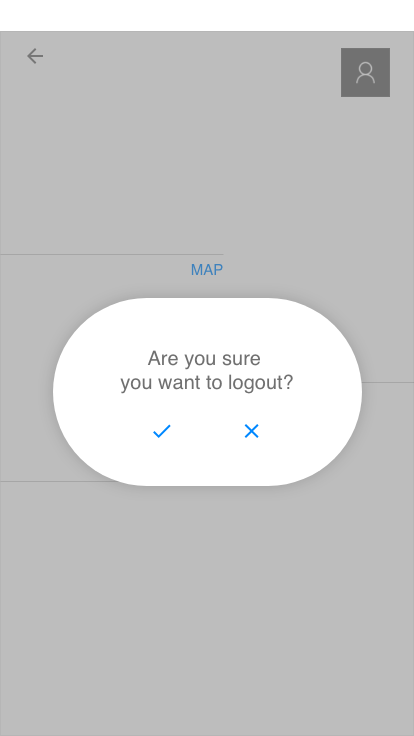
\includegraphics[width=60mm, height=100mm]{prototypes/ui/final/9.png} \\
(k) Artwork description & (l) Sign out \\[6pt]
\end{tabular}
\end{figure}

\newpage
\section{Technical Architecture}
\begin{figure}[H]
    \centering
    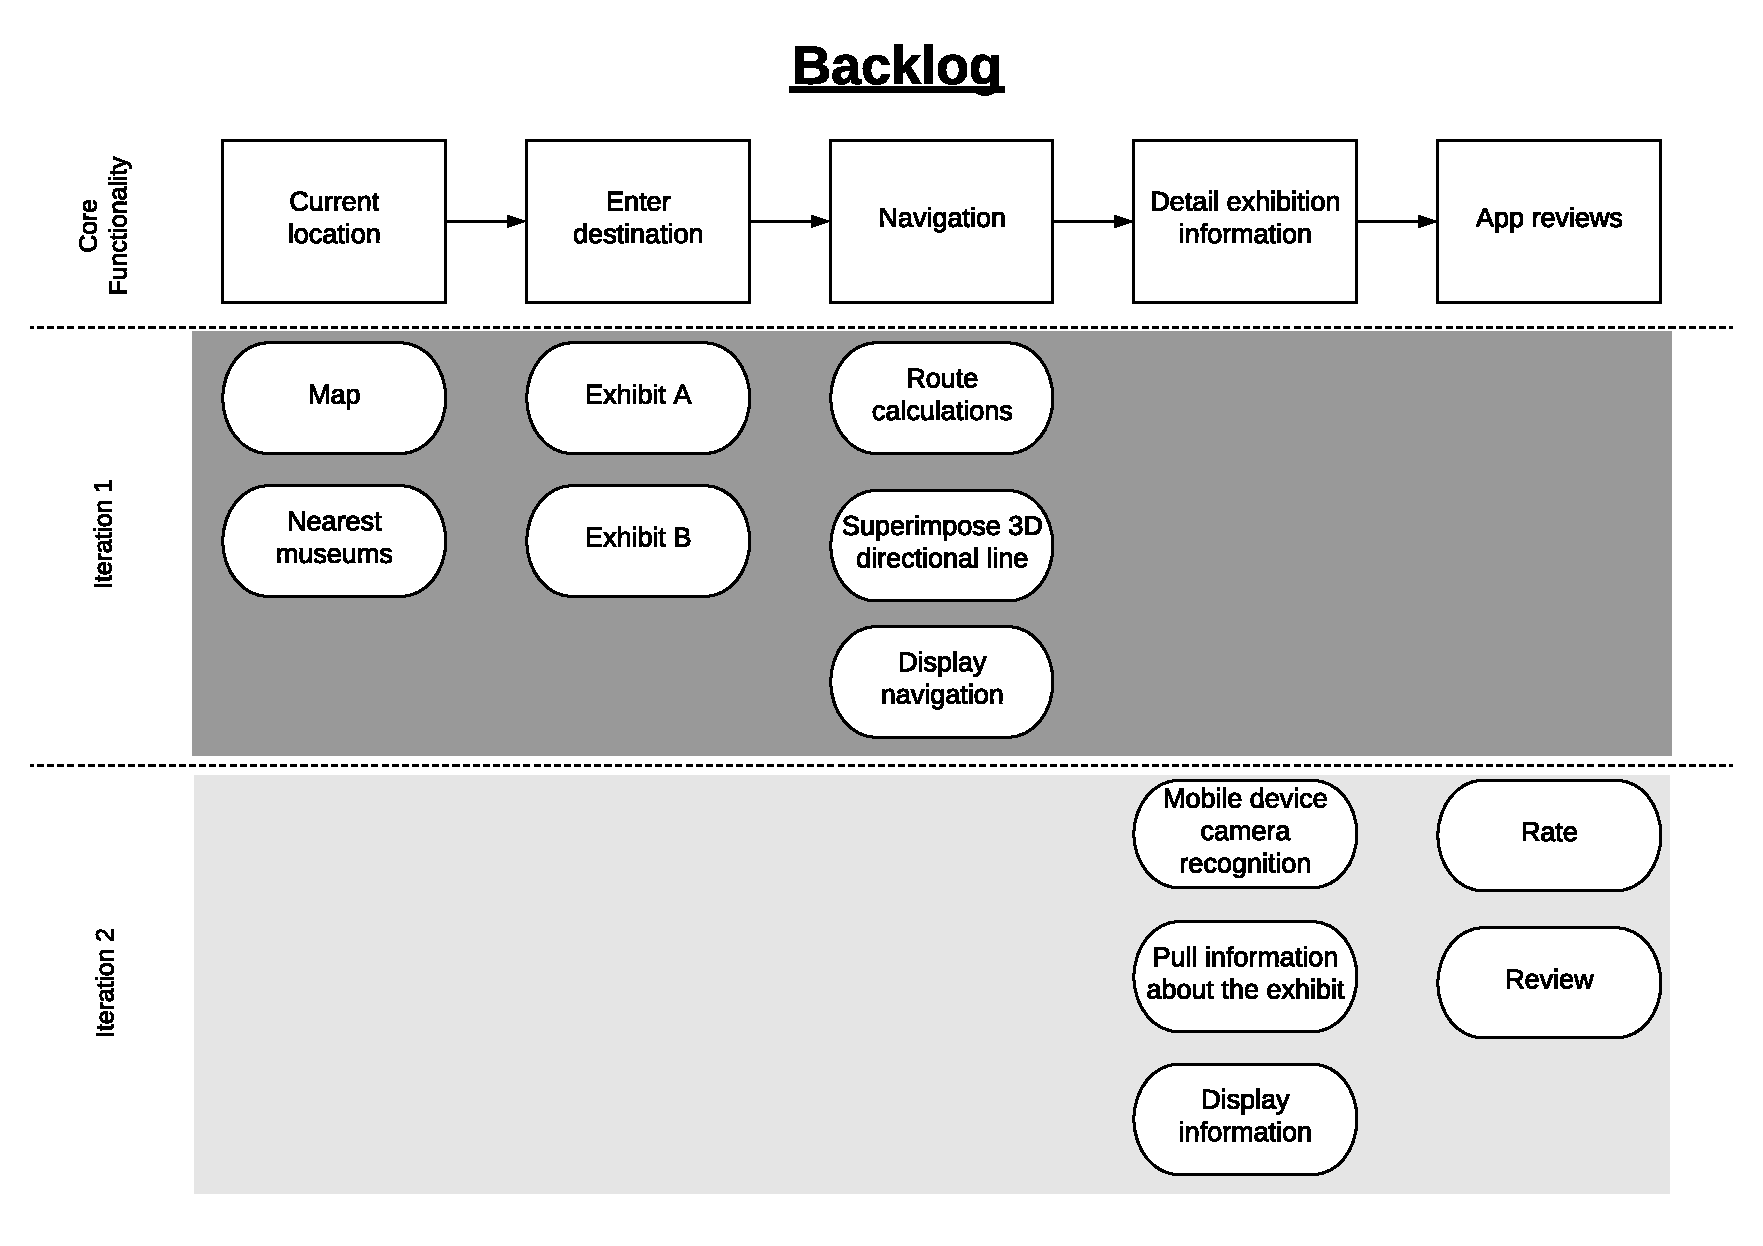
\includegraphics[width=\textwidth]
    {technicalarchitecture/backlog.pdf}
    \caption{Backlog Diagram}
    \label{fig:Backlog}
\end{figure}

\begin{figure}[H]
    \centering
    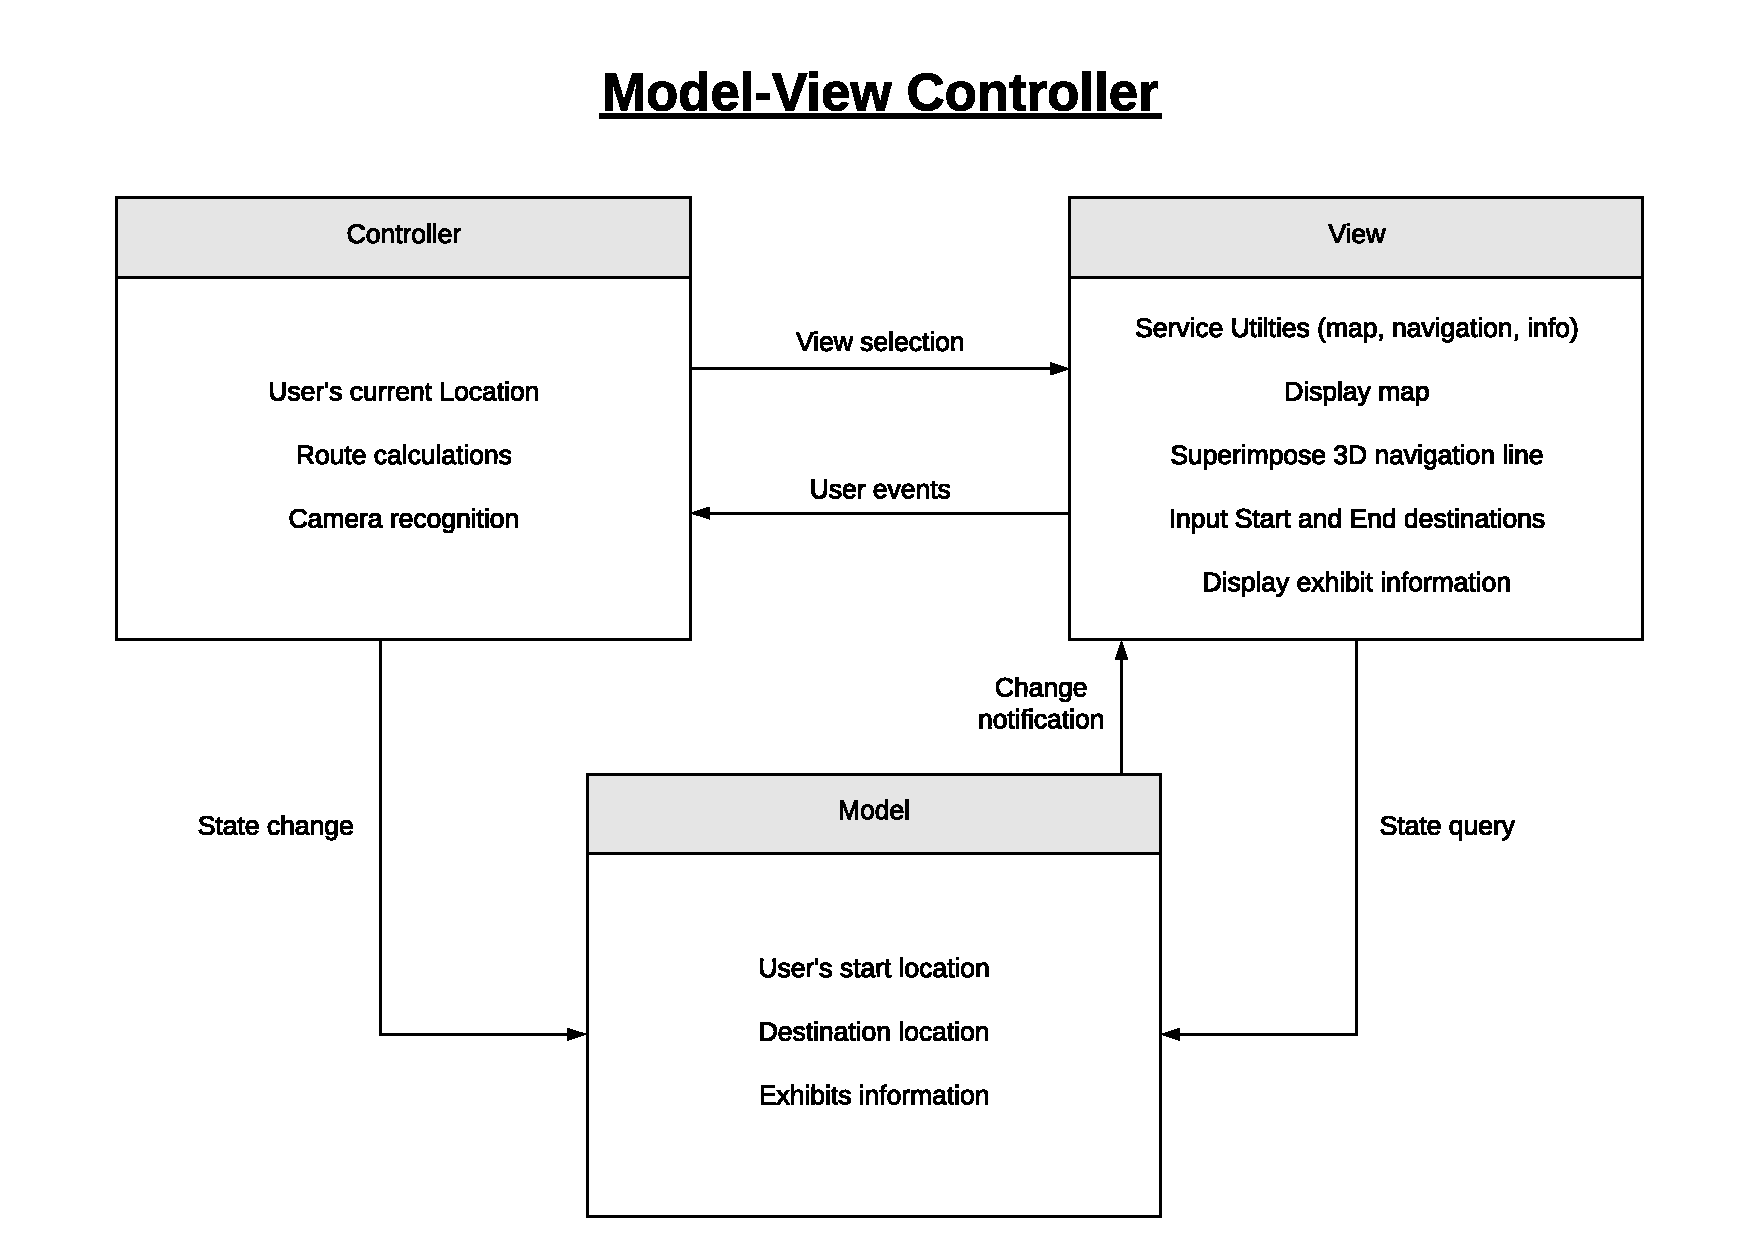
\includegraphics[width=\textwidth]
    {technicalarchitecture/mvc.pdf}
    \caption{Model-View Controller Diagram}
    \label{fig:MVC}
\end{figure}
